\documentclass[a4paper,twoside,kulak]{kulakreport}
% LATEX CLASSES
% Standaard: article, report, book, beamer, sciposter
% Huisstijl: kulakarticle, kulakreport, kulakbook, kulakbeamer, kulaksciposter

% PREAMBULE
% dit is het gedeelte tussen \documentclass en de \begin{document}
% hier worden extra pakketten geladen en instellingen gemaakt

% Essentiële pakketten aan het begin van de preambule om correct compileren mogelijk te maken
\usepackage[utf8]{inputenc} % Correct vreemde symbolen inlezen
\usepackage[dutch]{babel}   % Nederlandstalige regels voor woordafbreking
\usepackage[T1]{fontenc}    % Correct vreemde symbolen weergeven
\usepackage{float}
\usepackage{gensymb}
\usepackage{lscape}
\usepackage{rotating}
\usepackage{pdfpages}
\usepackage[square,numbers]{natbib}
\usepackage{siunitx}
\usepackage{hyperref}
\usepackage{amssymb}
\usepackage{booktabs}
\bibliographystyle{abbrvnat}


% Instellingen voor titelpagina, kop- en voettekst
% In een standaard article-document zijn er minder mogelijkheden
\faculty{Wetenschap \& Technologie Kulak}
\group{}
\title{Human Pose Estimation met OpenPose: een toepassing}
\subtitle{}
\author{Isaac Venus\\Stan Vanhecke\\Mathieu Vanooteghem}
% \\Stan Vanhecke\\Mathieu Vanooteghem
\emailaddress{isaac.venus@student.kuleuven.be}
% \\stan.vanhecke@student.kuleuven.be\\mathieu.vanooteghem@student.kuleuven.be
\institute{KU Leuven Kulak, Wetenschap \& Technologie}
\date{Titularis: Koen Van Den Abeele\\Begeleider: Jens Goemaere\\Academiejaar 2020 -- 2021}
\address{
   KU Leuven Kulak           \\
   Wetenschap \& Technologie \\
   Etienne Sabbelaan 53, 8500 Kortrijk             \\
   Tel.\ +32 56 24 60 20     \\
   \href{mailto:\theemailaddress}{\texttt{\theemailaddress}}
   }

\begin{document} % hier begint de eigenlijke inhoud van het document

\titlepage

\tableofcontents

\chapter*{Inleiding}
Aan materiaal in de paramedische wereld hangt vaak een stevig prijskaartje. Wij vroegen ons af hoe we deze kost kunnen verlichten en verschillende medische toepassingen gemakkelijker beschikbaar kunnen maken voor de gewone burger. Daarom maken we gebruik van technologie die iedereen ter beschikking heeft: een laptop of een smartphone.
In dit verslag richten wij ons op \emph{human pose estimation} (HPE), of lichaamspositiebepaling. We gebruiken hiervoor de open-source HPE software OpenPose die via neurale netwerken de positie van een persoon schat op een foto en de coördinaten van verschillende knooppunten in het menselijk lichaam teruggeeft waarmee we dan berekeningen kunnen uitvoeren. We zullen OpenPose gebruiken voor verschillende toepassingen met als doel een goede en goedkope oplossing aan te bieden die gemakkelijk toegankelijk is voor iedereen.

\chapter{Theoretische achtergrond}
\section{HPE, revolutionair?}
\emph{Human pose estimation} is de laatste tijd geëvolueerd naar een heel gebruiksvriendelijke vorm. Vroeger waren hier hoogtechnologische opstellingen met mensen in speciale pakken en veel rekenkracht voor nodig. Nu zijn een foto en een laptop voldoende om de posities van zelfs meerdere personen in hetzelfde beeld tegelijkertijd te bepalen. Dit allemaal door de gigantische vooruitgang op vlak van artificiële intelligentie en neurale netwerken.

Een 3D \emph{motion capture}-pak zorgt wel nog altijd voor een preciezere lichaamspositiebepaling dan de schatting die OpenPose maakt. Daarom wordt dit nog altijd gebruikt bij producties met een groot budget zoals films en games (zie Figuur \ref{3D_pak}).

	\begin{figure}[H]
		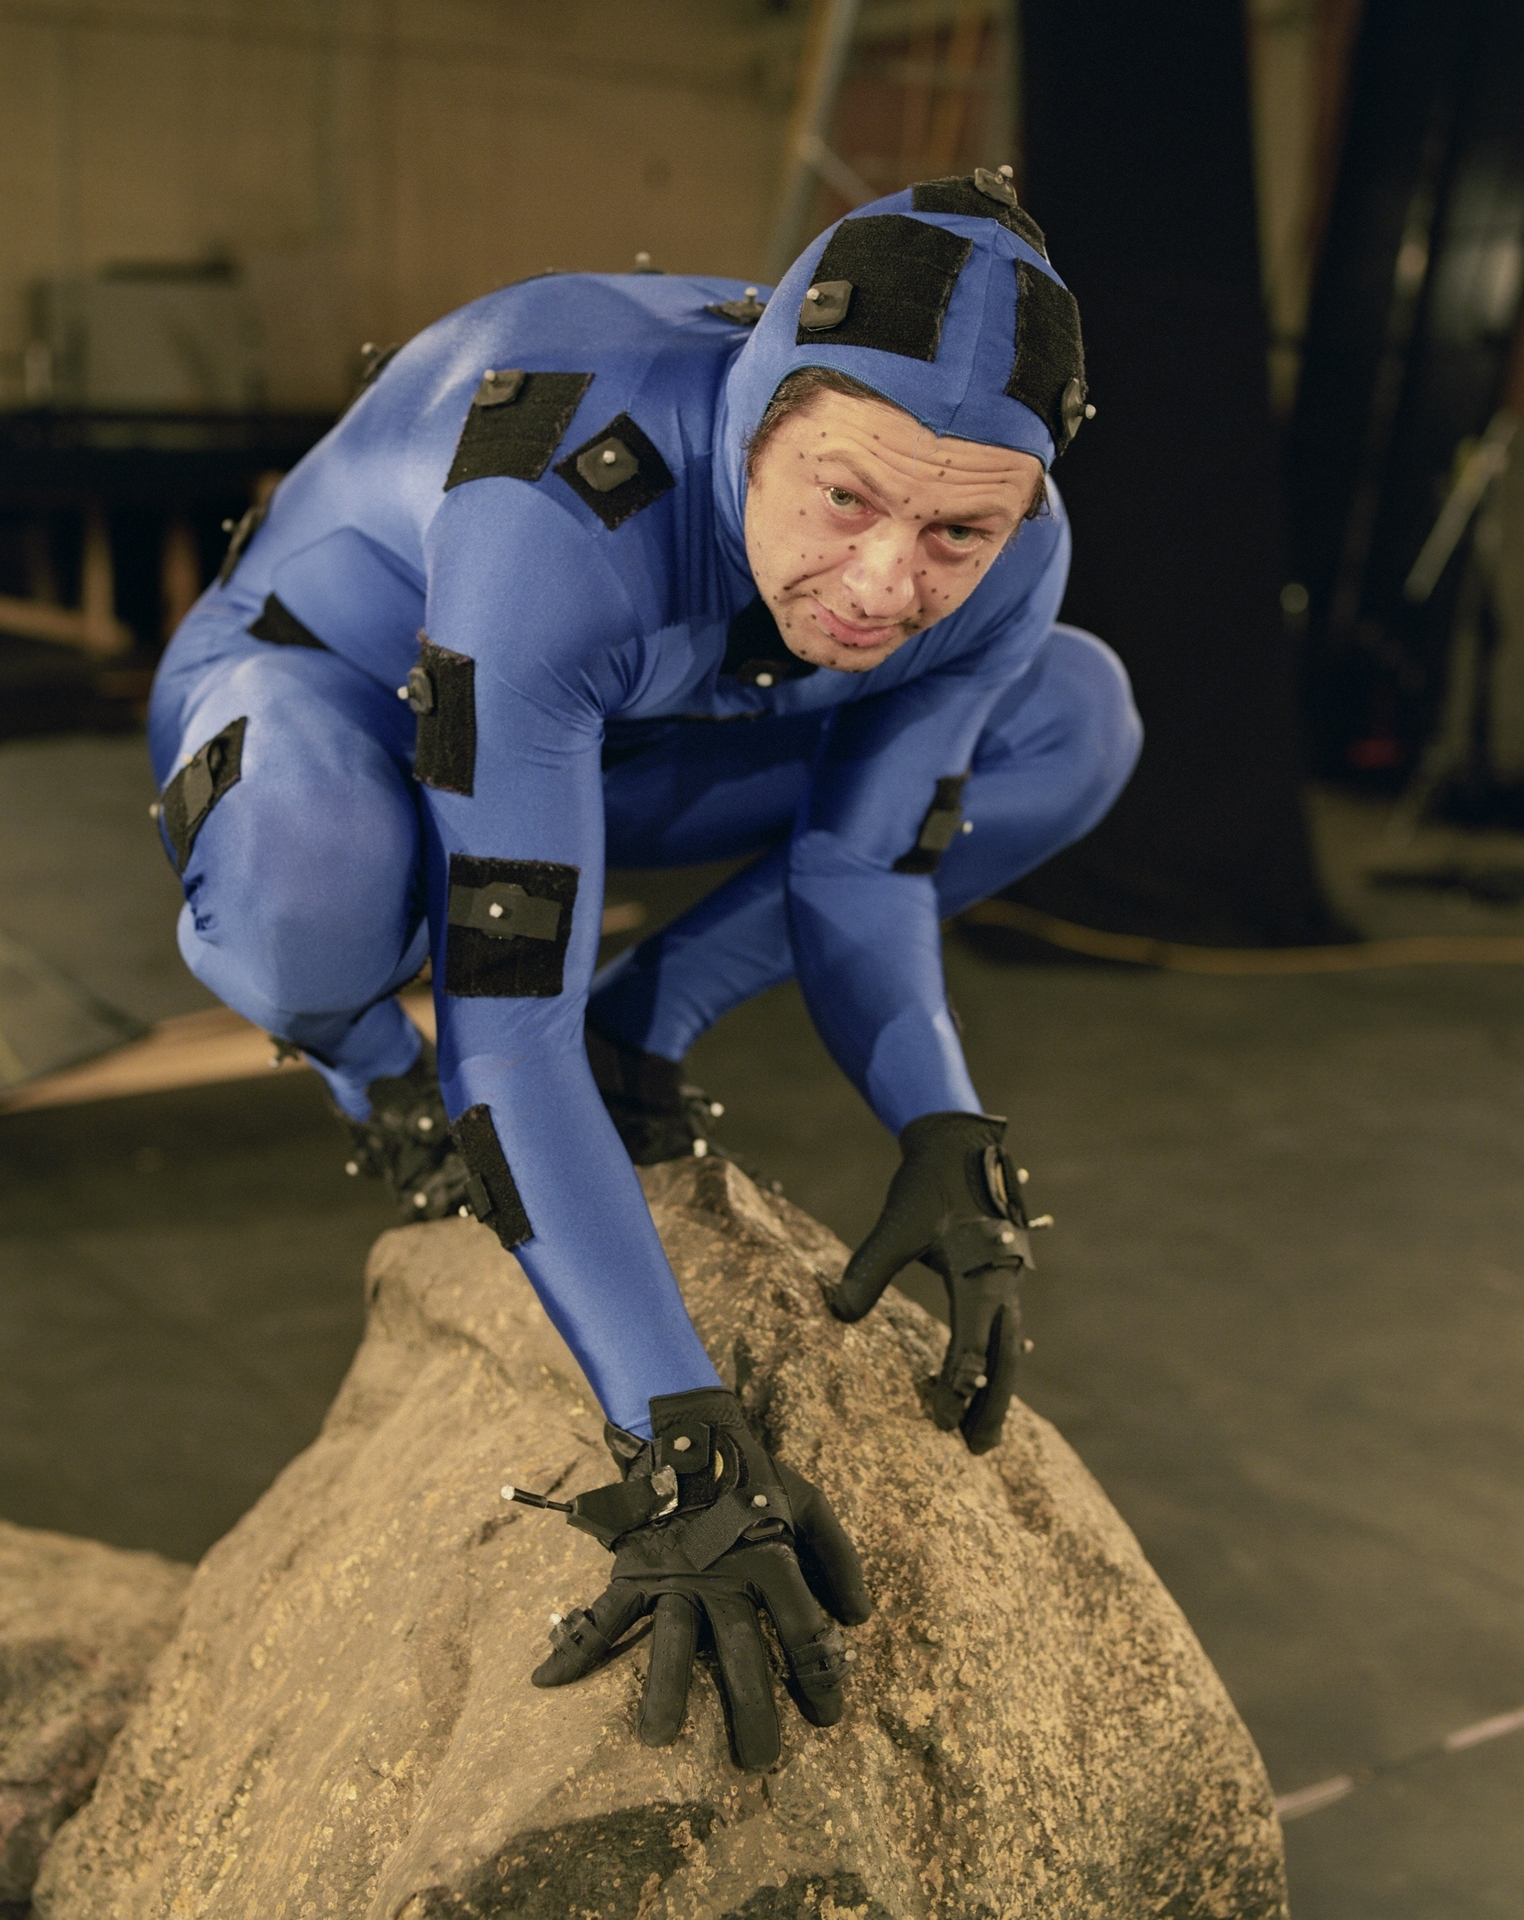
\includegraphics[width=.4\textwidth]{3D_motion_capture}
		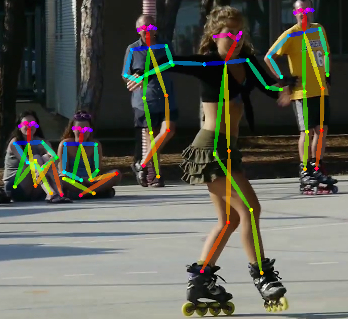
\includegraphics[width=.55\textwidth]{HPE_voorbeeld}
		\caption{Bij grote productiehuizen wordt de positie bepaald door middel van een 3D \emph{motion capture} pak (links), maar tegenwoordig is HPE een veel goedkopere en gemakkelijkere oplossing (rechts).
		(afbeeldingen van \href{https://www.pinterest.com/pin/718324209297102981/}{Pinterest} en \href{https://beyondminds.ai/an-overview-of-human-pose-estimation-with-deep-learning/}{beyondminds.ai})}
		\label{3D_pak}
	\end{figure}
\section{Neurale netwerken}
Een (artificieel) neuraal netwerk of ANN is een netwerk geïnspireerd op een biologisch neuraal netwerk zoals dat voorkomt in de hersenen, met als doel hen iets te doen leren. Het ANN is opgebouwd uit artificiële neuronen die neuronen in een brein moeten voorstellen. Al de neuronen zijn verbonden met andere neuronen en kunnen signalen uitsturen en ontvangen. In een ANN zijn de signalen getallen en kan elk neuron een bepaalde bewerking uitvoeren op een binnenkomend signaal om deze verder te sturen. Elke connectie heeft ook een gewicht dat bepaalt hoe sterk het signaal is dat hij uitstuurt. Dit gewicht past zich aan als het neuraal netwerk leert. 

\subsection{Opbouw van een neuraal netwerk}
\paragraph{Neuronen}
Zoals er hierboven staat, is een artificieel neuron geïnspireerd op een neuron uit een brein. Elk neuron heeft een of meerdere inputs en één output die kan verzonden worden naar meerdere andere neuronen. De input van een neuron kan ofwel komen van de data die aan het neuraal netwerk wordt gevoerd of van andere neuronen. De output van de outputneuronen is wat uit het programma komt. Om de output van een neuron te berekenen neem je de gewogen som van de inputs, met als gewicht de waarden van de connecties. Daarbij wordt ook nog eens een \emph{bias} of vertekening opgeteld.

\paragraph{Connecties}
Om te kunnen leren moet het natuurlijk mogelijk zijn om de data door te geven van het ene neuron naar het andere. Dit verloopt via een “connectie” die een bepaald gewicht heeft dat de sterkte en daarmee ook het belang van een bepaalde connectie weergeeft.

\paragraph{Lagen}
Een neuraal netwerk bestaat uit meerdere lagen van neuronen, meer bepaald de \emph{input layer}, \emph{hidden layers} en \emph{output layer} \ref{netwerk}. Zoals de namen wel duidelijk maken geef je de data aan de \emph{input layer} en komen de berekende waarden uit de \emph{ouput layer}. Daartussen zijn er eventueel \emph{hidden layers}. Tussen twee lagen zijn er meerdere manieren van connecties tussen de neuronen mogelijk.

\begin{figure}
	\begin{center}
		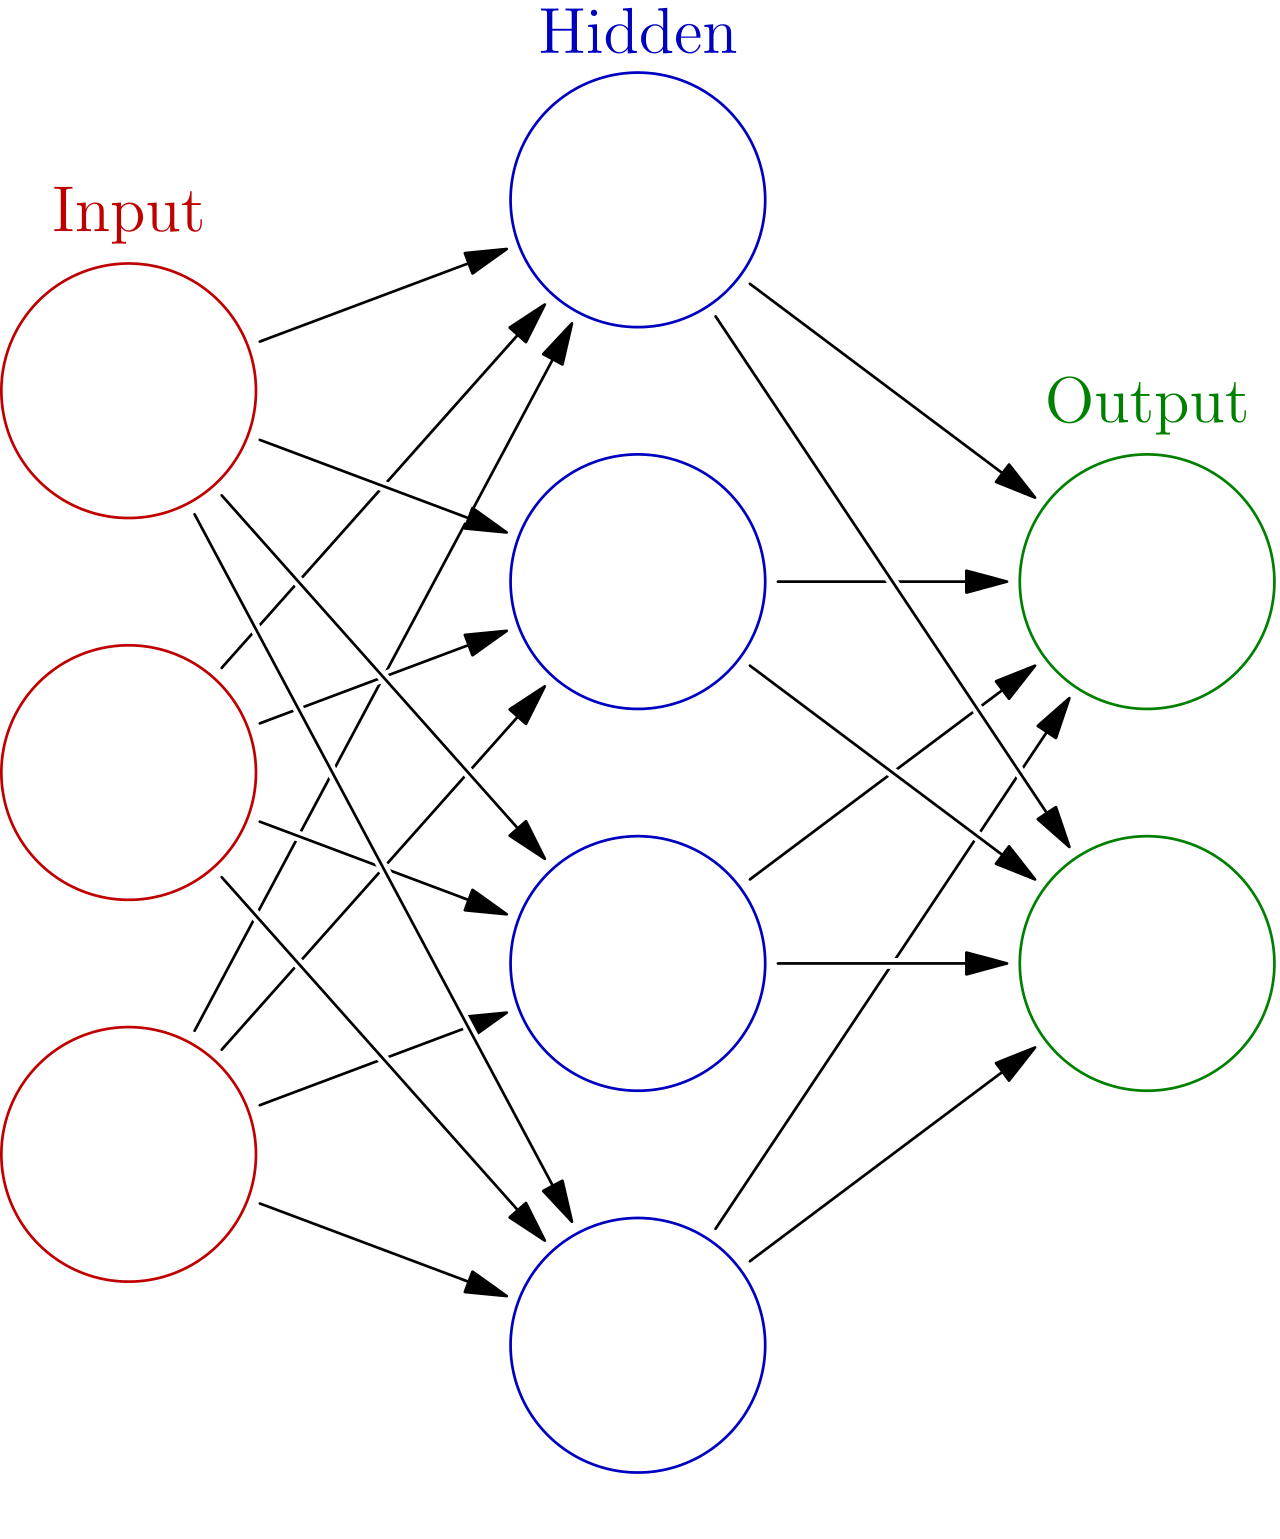
\includegraphics[width=8cm]{netwerk.png}
	\end{center}
	\caption{Voorbeeld van een neuraal netwerk. (afbeelding van \href{wikipedia.org}{Wikipedia})}
	\label{netwerk}
\end{figure}

\subsection{Trainen van een neuraal netwerk}
Bij het programmeren van een neuraal netwerk weet je natuurlijk niet wat de gewichten zijn van alle connecties. Je moet het model dus doen leren. Dit doe je door de gewichten (over meerdere leercycli) aan te passen zodat de output zo goed mogelijk past bij het gewenste resultaat. Er zal altijd een bepaalde fout op de output zitten dus het model zal nooit perfect zijn. Het trainen van een model is voltooid als de fout op de output niet meer verkleint en dus een minimum heeft bereikt. Het aanpassen van de gewichten gebeurt met een zekere \emph{learning rate}. Dit bepaalt de grootte van de correcties die gebeuren bij de gewichten. Bij een grote \emph{learning rate} kan je model sneller klaar zijn met leren, maar is er meer kans op een grotere fout op de output. Een kleine \emph{learning rate} zal het trainen vertragen maar je uiteindelijke resultaat zal beter zijn. OpenPose is getraind met twee datasets \cite{openpose}: de COCO dataset, die bestaat uit meer dan 100.000 beelden en meer dan 1.000.000 \emph{keypoints}, en de MPII dataset.
\section{OpenPose}

Over het algemeen zijn er 2 manieren om menselijke poses te schatten. Ten eerste heb je de \textit{top-down} aanpak. Hierbij maak je eerst gebruik van een personendetector en schat je dan voor elke persoon apart hun \emph{pose}.  Deze methode heeft enkele minpunten, namelijk dat de looptijd evenredig is met het aantal personen en als een persoon in de eerste stap niet herkend wordt, is er geen mogelijkheid om de fout toch nog goed te maken. Een \textit{bottom-up} aanpak daarentegen heeft deze problemen niet. Deze methode bepaalt alle belangrijke knooppunten en probeert dan de punten op de juiste manier aan elkaar te linken zodat het de poses van verschillende mensen vormt. OpenPose is een voorbeeld van zo’n \textit{bottom-up} aanpak en is een van de meest efficiënte neurale netwerken voor positiebepaling. OpenPose was de eerste open-source software voor realtime lichaams-, voet-, hand- en gezichtsdetectie. Het maakt gebruik van een “\textit{two-branch multistage} CNN”, heel kort betekent dit het volgende: CNN staat voor convolutioneel neuraal netwerk, “\textit{two-branch}” wijst op het feit dat het CNN twee takken heeft en \textit{multistage} wil zeggen dat het netwerk meerdere keren op elkaar is gestapeld. Op figuur \ref{algoritme} zie je de architectuur van het netwerk.

\subsection{Werking}

Het systeem neemt een kleurenfoto met grootte $w \times h$ als input en geeft als output voor elke persoon op de foto de 2D-locaties van zijn lichaamsdelen. Eerst wordt een eerste voorspelling gedaan van de set van 2D-vectorvelden ($\textbf{L}$). Dit zijn \textit{part affinity fields} (PAF's), zij leggen de graad van associatie tussen de lichaamsdelen vast. Ook van de 2D- etrouwbaarheidskaarten ($\textbf{S}$) van de lichaamsdelen wordt een eerste schatting gedaan. Dit zijn respectievelijk de eerste en de tweede tak van het CNN. Deze eerste voorspelling wordt dan door het netwerk verbeterd. Vervolgens wordt deze verbeterde voorspelling samen met de initiële voorspelling nog eens gevoerd aan het netwerk. Na zes keer is het resultaat goed genoeg en wordt het samengevoegd om de uiteindelijke output te geven. Omdat het netwerk meerdere keren doorlopen wordt, noemt men dit een \textit{multistage} CNN. De volledige uitleg van het netwerk en hoe men van de heatmaps en PAF's tot het uiteindelijke resultaat komt, vind je in het origineel artikel.\cite{openpose}

\begin{figure}[H]
	\centering
	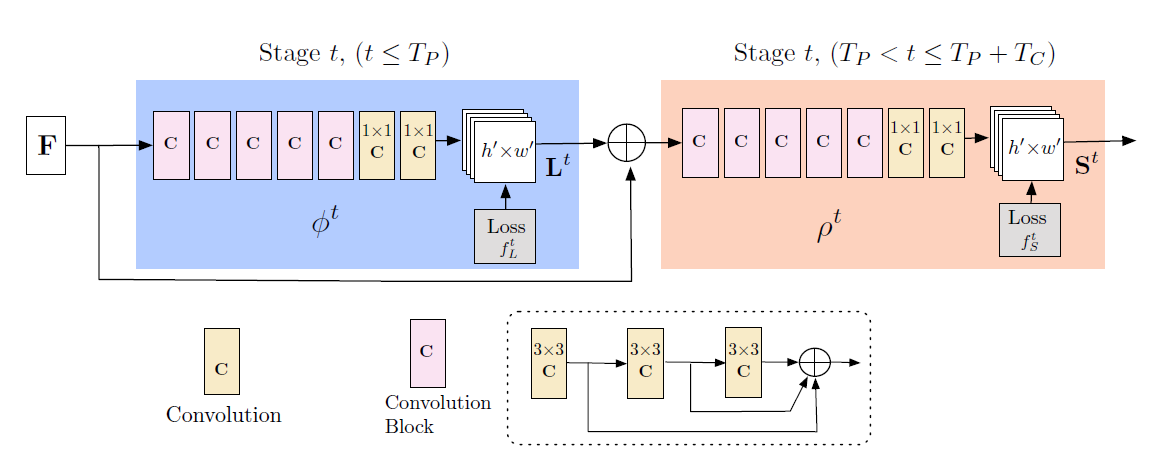
\includegraphics[width=0.8\textwidth]{algoritme_architectuur}
	\caption{Architectuur van het CNN. De eerste set stappen voorspelt de PAF's, terwijl de tweede set de betrouwbaarheidskaarten voorspelt. De voorspellingen van elke stage worden dan aaneengeschakeld voor elke volgende stage. \cite{openpose}}
	\label{algoritme}
\end{figure}

De set \textbf{L} bestaat uit $C$ vectorvelden, één per connectie tussen twee knooppunten, $\textbf{L} = (\textbf{L}_1,\textbf{L}_2,...,\textbf{L}_C)$. Elke $\textbf{L}_c \in \mathbb{R}^{w \times h \times 2}$ , met $c \in \{1...C\}.$ De PAF’s  zijn velden die de graad van associatie representeren tussen de verschillende lichaamsdelen. Er wordt gestart met een set van connecties tussen twee punten. Voor elke connectie wordt dan zo’n veld opgesteld. Het is eigenlijk een tensor met in elke cel een 2D-vector die de richting van de connectie aangeeft, bijvoorbeeld van de rechterschouder naar de rechterelleboog.
De set $\textbf{S} = (\textbf{S}_1,\textbf{S}_2,...,\textbf{S}_j)$ bestaat dus uit $\textbf{J}$ betrouwbaarheidskaarten, één per lichaamsdeel en $\textbf{S}_j \in \mathbb{R} ^{w \times h}$ , $j \in \{1...J\}$.
Deze worden heel duidelijk voorgesteld met heatmaps. Hierop zie je voor elke positie de kans dat het lichaamsdeel zich daar bevindt. Indien er meerdere mensen op de foto staan, zal je meerdere punten zien met een hoge kans. Figuur \ref{heatmap} is bijvoorbeeld de heatmap voor de rechterelleboog. Er zijn duidelijk vier zone's met hoge kans zichtbaar. De zone helemaal links heeft geen rood, dit wijst op een laag vertrouwen dat het juist is. Dit komt doordat de elleboog niet duidelijk zichtbaar is.

Zoals eerder gezegd worden uiteindelijk de betrouwbaarheidskaarten en PAF's samengevoegd om als output de 2D-knooppunten van alle mensen op de foto te geven.

\begin{figure}
	\centering
	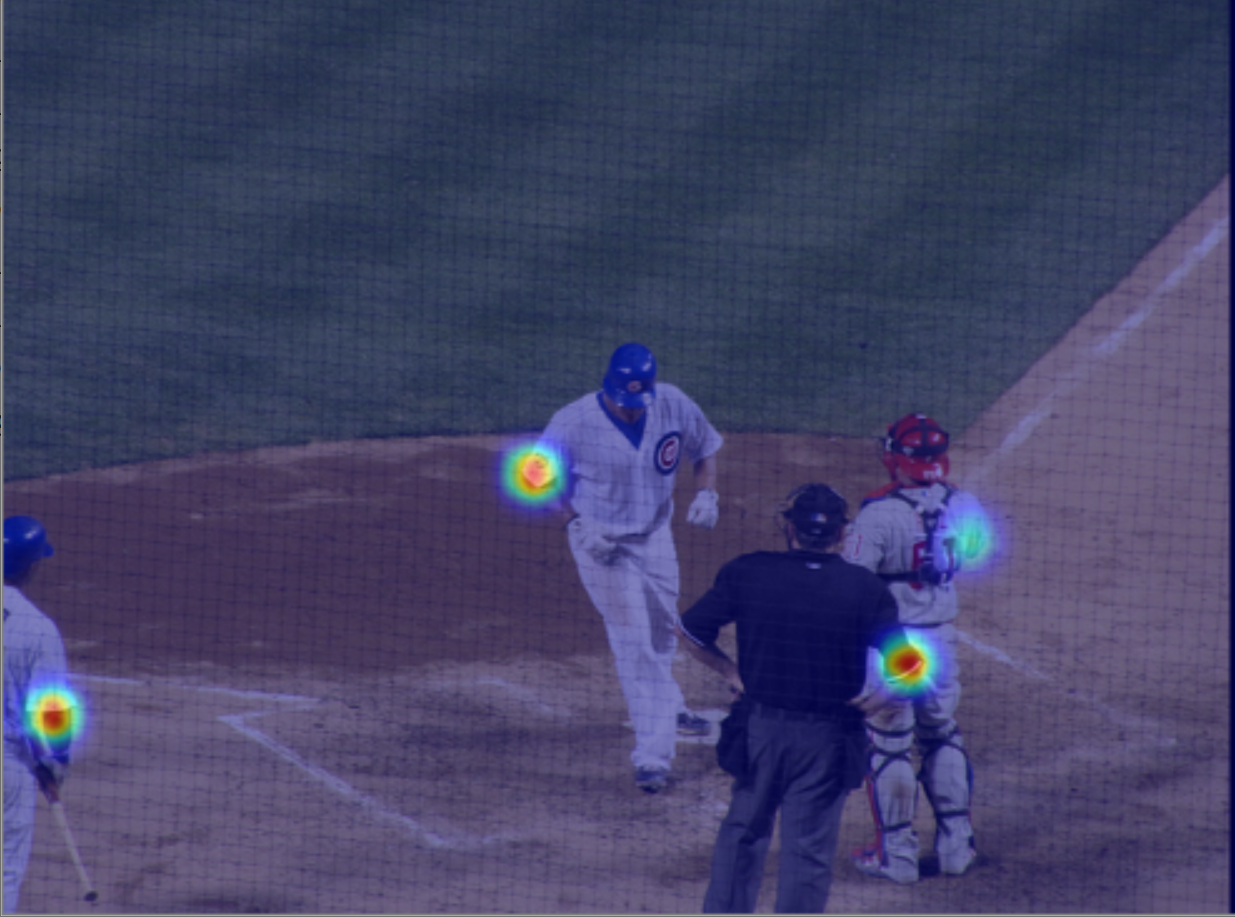
\includegraphics[width=0.8\textwidth]{heatmap_1}
	\caption{Dit is de heatmap voor de rechterelleboog. Je ziet dat de elleboog van de meest rechtse persoon niet heel duidelijk zichtbaar is, de voorspelling in dat punt heeft daarom een lage zekerheid. Figuur uit \href{https://github.com/CMU-Perceptual-Computing-Lab/openpose}{OpenPose}.}
	\label{heatmap}
\end{figure}


\chapter{Toepassingen}
Zoals eerder al gezegd zullen we ons focussen op toepassingen in de paramedische wereld waarop HPE kan toegepast worden. Wij proberen hiervoor dan een goedkope oplossing te ontwikkelen. Hierbij testen we mogelijke problemen en analyseren we of dit  een goede optie is. We proberen dit dan allemaal op een methodische manier uit te werken, waarbij we een specifiek geval steeds breder gaan bekijken.

Een eerste toepassing is het opvolgen van de revalidatie na een schouderoperatie. Met een foto gemaakt met een gsm kunnen we een analyse uitvoeren van de beweeglijkheid van de schouder na de operatie en dan doorheen de revalidatie opvolgen.

Een tweede en uitgebreidere toepassing is het analyseren van de positie op de fiets. Veel amateurwielrenners hebben een slechte houding op de fiets en een professionele \emph{bikefitting} kost al snel een paar honderd euro. Via lichaamspositiebepaling kunnen wij met een simpele foto de positie bepalen op de fiets en dan correcties voorstellen. Dit is een goedkope oplossing die voor een zeer breed publiek inzetbaar is. Voor professionele wielrenners zal dit waarschijnlijk niet voldoende zijn, maar voor een amateur kan dit een goedkoop alternatief zijn.

Tenslotte analyseren we via een filmpje het uitvoeren van fitnessoefeningen. Hier hebben we specifiek gekozen voor een squat, maar het concept is breder inzetbaar voor andere oefeningen. Het slecht uitvoeren van oefeningen kan op termijn leiden tot blessures. Ook kost een personal trainer al snel veel geld en moet die altijd ter plaatse zijn om te bepalen of je een bepaalde oefening correct uitvoert. Met behulp van OpenPose kunnen we dit nu virtueel bepalen met een filmpje van de oefening als input.

Al de programma's die geschreven werden voor de toepassingen zijn te vinden op \href{https://github.com/isaacvenus/LPB}{Github}

\section{Toepassing 1: opvolgen van revalidatie na schouderoperatie}
\subsection{Bepalen van de hoek tussen arm en lichaam}

We willen meten hoe ver een persoon zijn arm kan roteren voor de opvolging van de revalidatie na een schouderoperatie. Hiervoor kunnen we de hoek tussen het opperarmbeen en de romp bepalen. We gaan ervan uit dat deze hoek het meest relevant is voor het meten van de beweeglijkheid van de schouder. Op figuur~\ref{fig:skelet} komt dat dus neer op de hoek bepalen tussen de lijnstukken [3,2] en [2,1] of tussen de lijnstukken [1,5] en [6,5]. Als we OpenPose gebruiken om de positie te schatten van een persoon op een foto krijgen we als output de coördinaten van de verschillende knooppunten. Met deze coördinaten hebben we voldoende informatie om de hoek te berekenen en zo objectieve informatie te krijgen over het verloop van de revalidatie.

Bij een foto vanuit vooraanzicht kunnen we berekenen hoe ver de patiënt zijn arm zijwaarts omhoog kan brengen. Bij een foto genomen vanuit zijaanzicht kunnen we berekenen hoe ver hij de arm vooruit omhoog kan brengen. Het is wel belangrijk dat de foto altijd vanuit dezelfde positie wordt genomen omdat er anders variatie kan zijn op de hoek.



\begin{figure}[H]
	\centering
	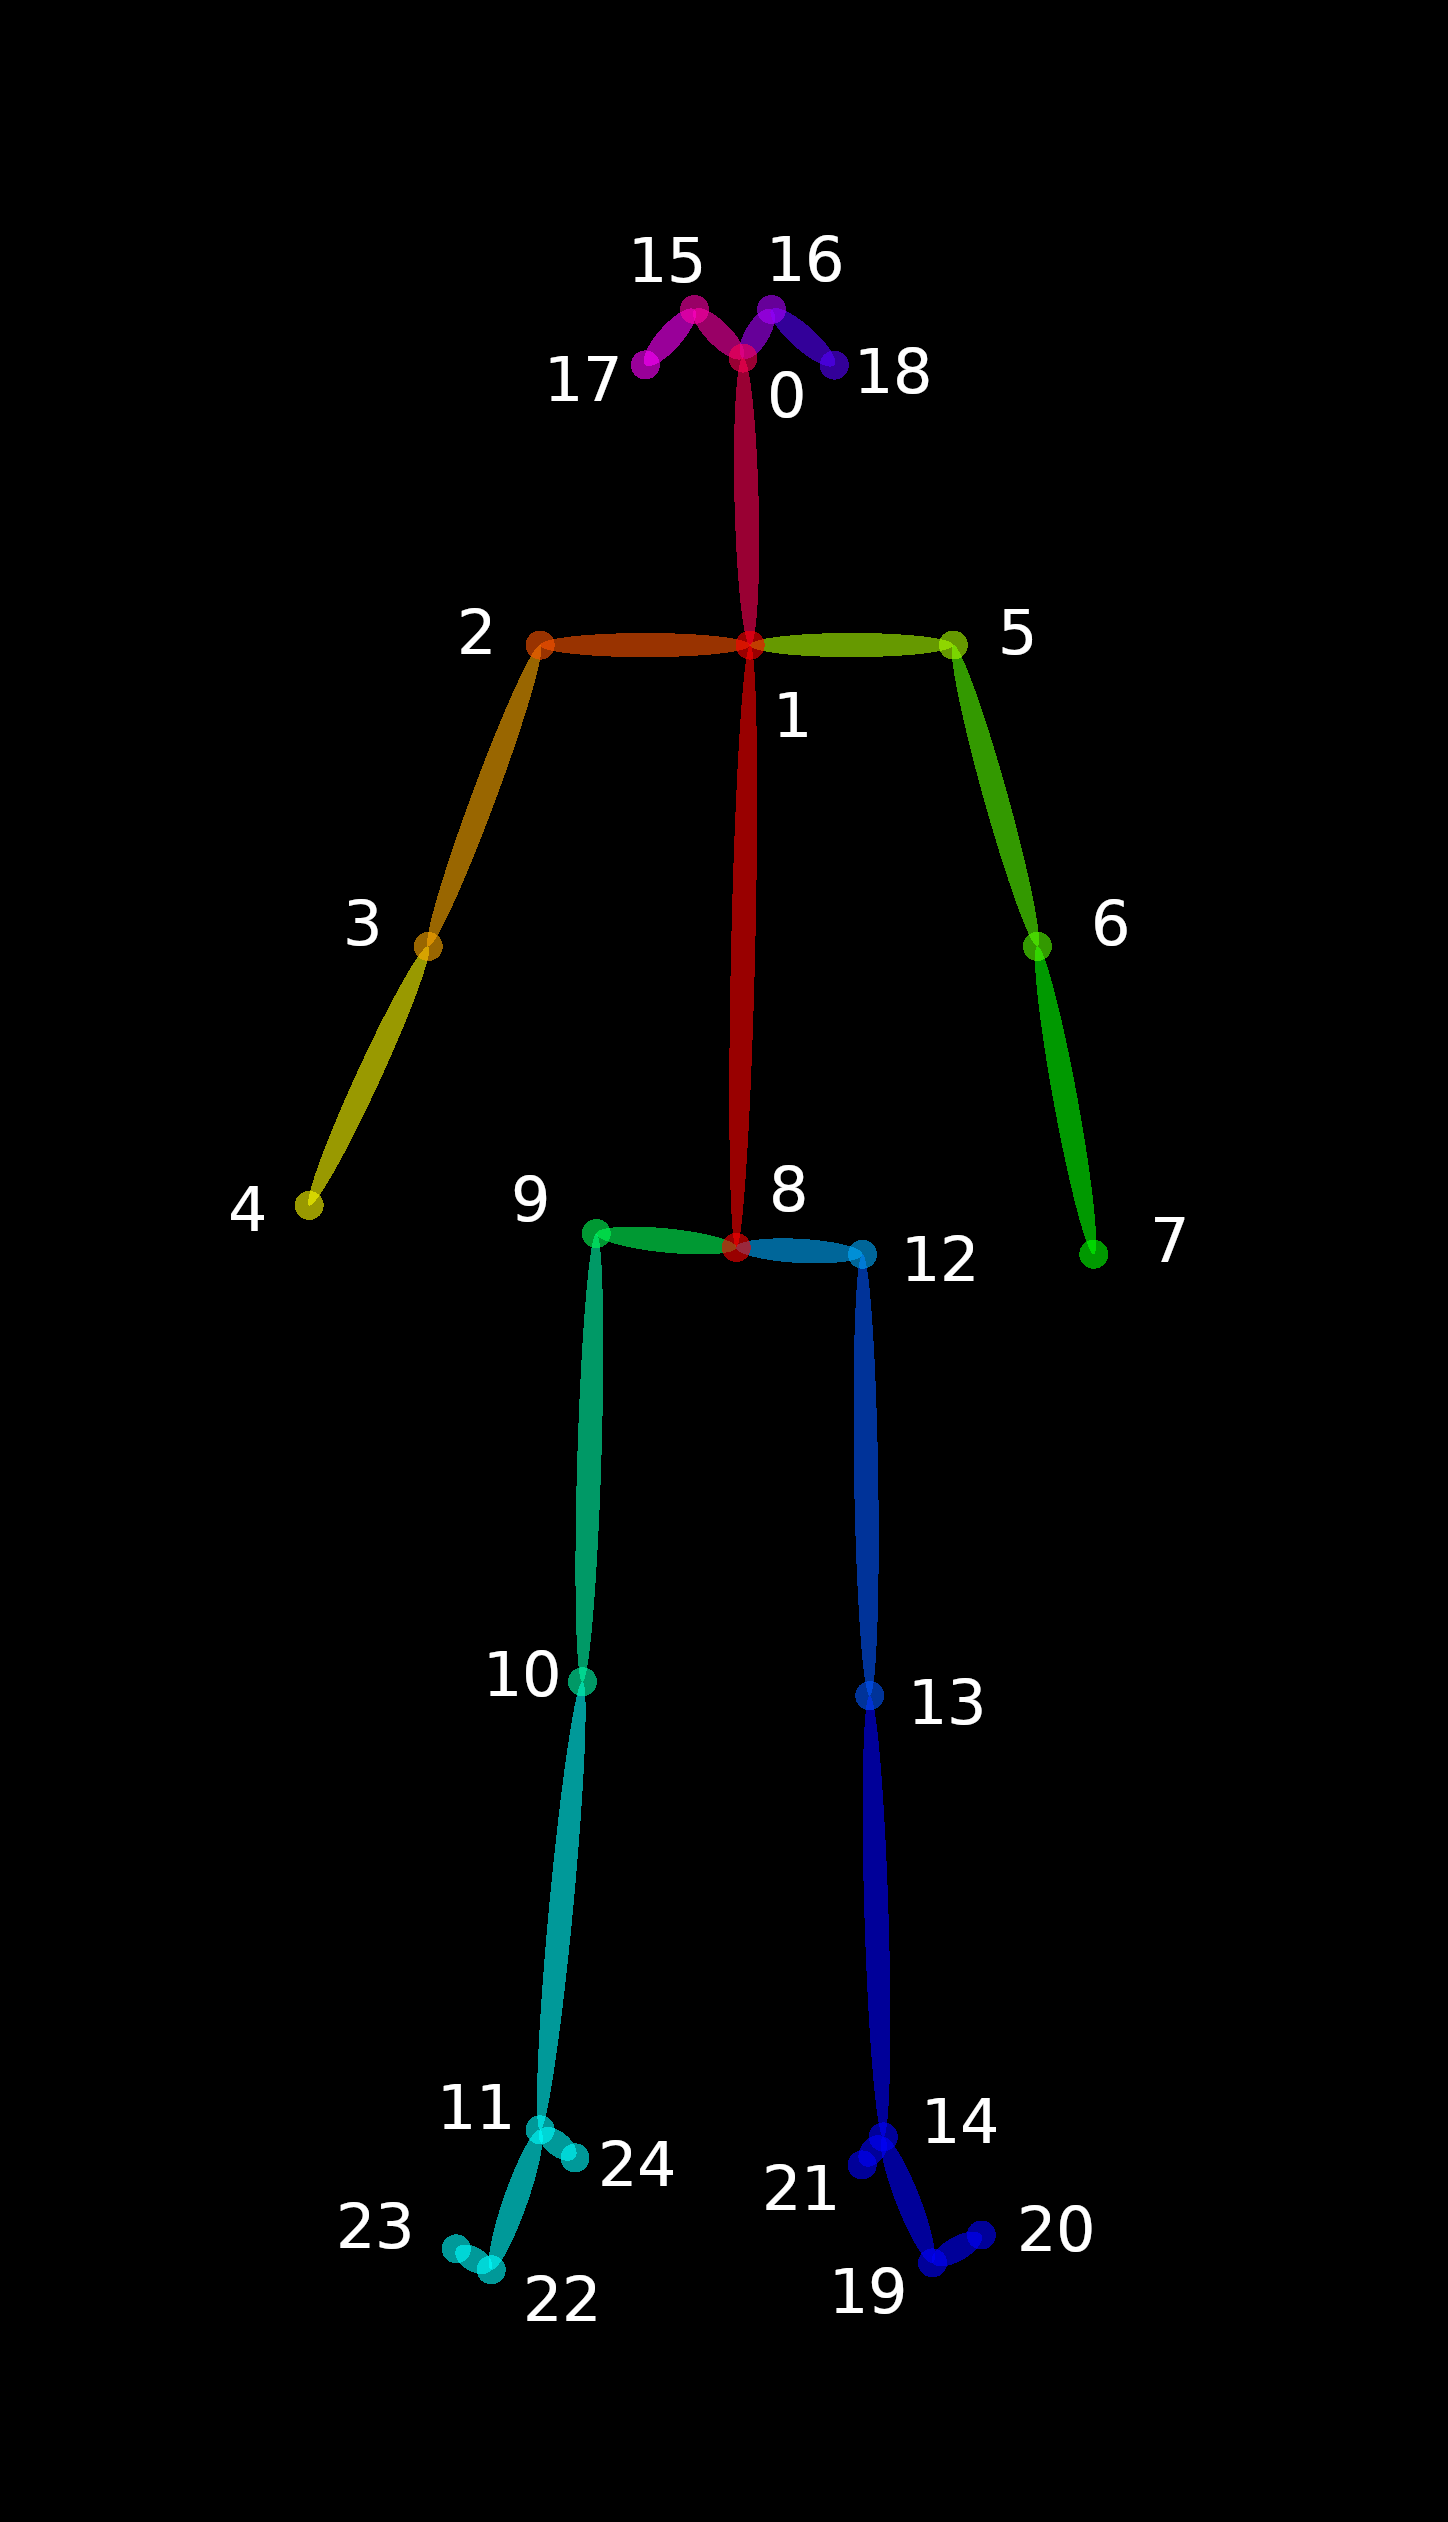
\includegraphics[width=.5\textwidth]{HPE_skelet}
	\caption{Voorstelling van de positie bepaald via OpenPose (afbeelding van \href{https://github.com/CMU-Perceptual-Computing-Lab/OpenPose/blob/master/doc/output.md}{OpenPose})}
	\label{fig:skelet}
\end{figure}


\subsection{Resultaten}

We krijgen de coördinaten van alle punten die OpenPose kan herkennen. Hiermee kunnen we dan verder onderzoek doen. Op dit moment zijn we in staat om hoeken tussen bepaalde lichaamsdelen te berekenen met als doel objectieve gegevens te bekomen tijdens bijvoorbeeld een revalidatie na een ongeval.

\paragraph{Wiskundige achtergrond}
Om de hoek tussen twee lichaamsdelen te berekenen gebruiken we de cosinusregel. Hier volgt een klein beetje duiding over hoe we die precies gebruiken (zie figuur \ref{cos}).\\

\begin{figure}[H]
	\begin{center}
		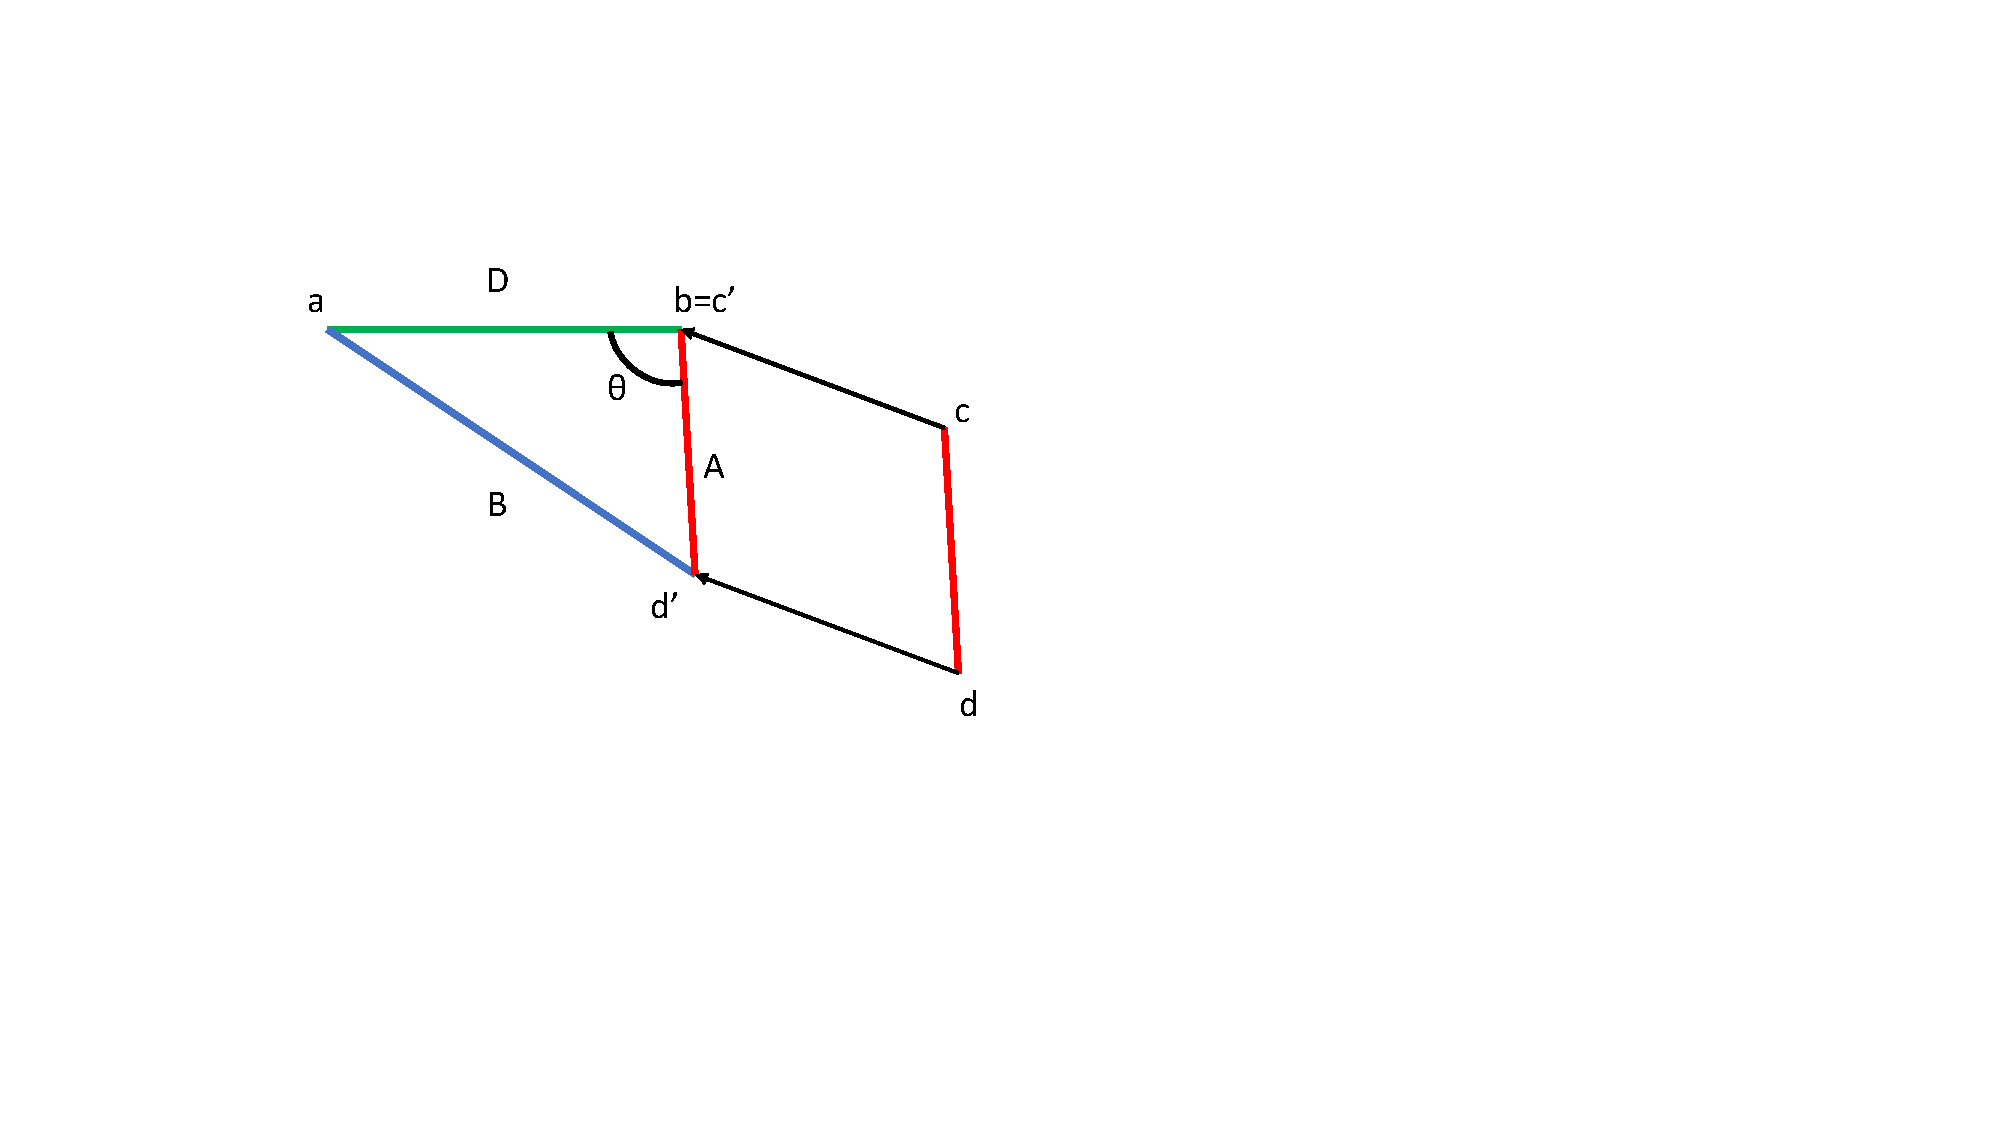
\includegraphics[width=10cm]{cos.pdf}
	\end{center}
	\caption{Hoek tussen 2 lichaamsdelen}
	\label{cos}
\end{figure}

We stellen \(a, b\) de coördinaten die het eerste lichaamsdeel afbakenen en \(c, d\) de coördinaten van het tweede lichaamsdeel. De hoek tussen de lichaamsdelen is dan de \(\theta\) van op de figuur. We kunnen gewoon de cosinusregel gebruiken om de hoek te bepalen als we \(c\) op \(b\) leggen. We krijgen dan
\[B^2 = A^2 + D^2 -2\cdot A\cdot D\cos\theta\]
en dus
\[\cos\theta = \frac{A^2 + B^2 - B^2}{2\cdot A\cdot D}\]
met
\[A = \sqrt{(d_x - c_x)^2 + (d_y - c_y)^2}\]
\[B = \sqrt{(b_x - a_x + d_x - c_x)^2 + (b_y - a_y + d_y - c_y)^2}\]
\[D = \sqrt{(b_x - a_x)^2 + (b_y - a_y)^2}\]
Als we dus de 4 coördinaten weten kunnen we de hoek bepalen.
\paragraph{Voorbeeld}
Een voorbeeld bij het bepalen van een hoek tussen de bovenarm en de romp is afbeelding \ref{samen}. Als we de hoek berekenen tussen de ruggengraat (rood) en het opperarmbeen(licht oranje) krijgen we als waarden:
\begin{itemize}
	\item Foto 1: 21.63 graden
	\item Foto 2: 78.06 graden
	\item Foto 3 130.00 graden
\end{itemize}
\begin{figure}
	\begin{center}
		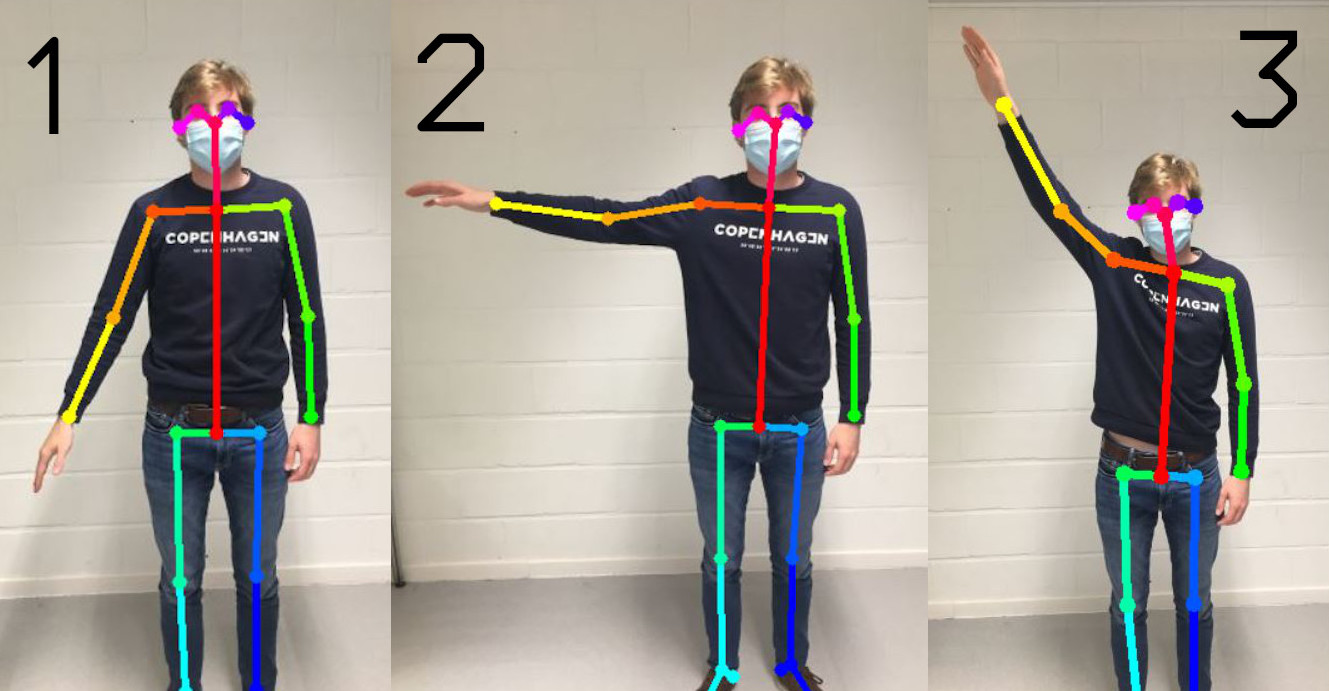
\includegraphics[width=12cm]{samen.jpg}
	\end{center}
	\caption{Voorbeeld bij het bepalen van een hoek.}
	\label{samen}
\end{figure}
\subsection{Conclusies}
Door deze  toepassing weten we dat het relatief eenvoudig is om met OpenPose zinvolle berekeningen te doen. We zouden dit programma nog verder kunnen uitwerken zodat het bruikbaar is voor bijvoorbeeld kinesisten. Door de coördinaten die gegeven worden als output kunnen we gemakkelijk programma's schrijven die hiermee werken. Doordat OpenPose werkt in 2D moeten de foto's wel recht genomen worden. Als de hoek die we willen berekenen schuin afgebeeld staat op de inputfoto komt de berekening niet overeen met de werkelijke waarde van de hoek. Meer informatie hierover in sectie \ref{camerapositie}.


\section{Toepassing 2: fietspositie bepalen}
Als tweede toepassing willen we onderzoeken of we een goedkoper alternatief kunnen bieden voor een \textit{bikefitting}. Hierbij worden er foto's genomen van de persoon op de fiets en kunnen we dan op basis van de positie bepaald met OpenPose eventuele correcties uitvoeren op de fiets.

Een \emph{bikefit} is eigenlijk het analyseren en eventueel aanpassen van de positie op de fiets. Het belangrijkste doel daarvan is het voorkomen van blessures. Bij wielrenners die aan competitie doen heeft een \emph{bikefit} ook als doel om een zo aerodynamisch mogelijke positie op de fiets aan te nemen. Ook kan een betere positie ervoor zorgen dat men een groter vermogen kan leveren op de pedalen. Alleen maar voordelen dus.

\subsection{Principe}

Op Figuur \ref{fig:bikefit} staan enkele hoeken die voor de doorsnee persoon als optimaal gezien worden voor de positie op een koersfiets. Deze hoeken kunnen wel wat variëren afhankelijk van hoe flexibel de persoon is. Met behulp van OpenPose berekenen we deze hoeken met als input een of meerdere foto's van de wielrenner. Het is belangrijk dat de foto genomen wordt vanuit een zo loodrecht mogelijk zijaanzicht en dat de wielrenner het stuur vasthoudt bij de \emph{shifters}. Ideaal wordt de foto getrokken op ongeveer de helft van de hoogte van de fietser als die zit. Als de berekende hoeken te veel afwijken van wat voorop gesteld wordt, dan kunnen we een verbetering voorstellen. Dit kan een verhoging van het zadel zijn of een verandering van de lengte van de stuurpen.


\begin{figure}[H]
	\centering
	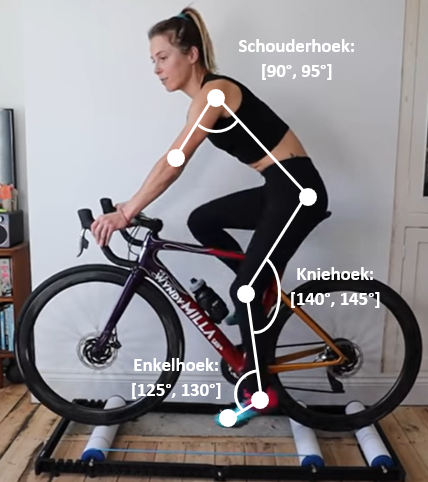
\includegraphics[width=\textwidth]{bikefit_hoeken_foto}
	\caption{Belangrijkste hoeken voor een optimale positie op de fiets (hoeken zijn gebaseerd op presentatie over bikefitting door Wolf Performance, bijgewoond door onze begeleider Jens Goemaere) (foto is een screenshoot van \href{https://www.youtube.com/watch?v=h7ZEaTmylXk}{Juliet Elliott op YouTube})}
	\label{fig:bikefit}
\end{figure}

\subsection{Algoritme voor wijzigen van de zadelhoogte}

We beginnen met een algoritme te schrijven voor het veranderen van één parameter, namelijk de zadelhoogte. Voornamelijk de kniehoek zal variëren als gevolg van een wijziging in zadelhoogte. Dit zal ook een klein effect hebben op de schouderhoek maar dit laten we hier voor het gemak achterwege. De mate waarin je de zadelhoogte kan wijzigen hangt af van de lengte van de zadelpen. Op de meeste zadelpennen staat de minimale diepte waarmee de pen in het frame moet zitten. Indien dit niet zo is, is de vuistregel dat de zadelpen minstens 90 \si{mm} diep in het frame moet zitten. Zet je zadel dus zeker niet hoger dan dat. Als je dit niet doet, bestaat de kans dat de zadelpen breekt.
Eerst berekenen we de kniehoek. We kijken initieel hoe groot die is en we weten welke hoek we willen bereiken. Deze ligt ideaal tussen 140\degree en 145\degree (zie Figuur \ref{fig:bikefit}). Het algoritme berekent dan met hoeveel pixels de y-coördinaat van het knooppunt van de heup moet wijzigen om de hoek te bekomen. Vooraf wordt door het programma de lengte van bijvoorbeeld het bovenbeen gevraagd in \si{cm}. Via OpenPose kunnen we dan het aantal pixels berekenen tussen het knooppunt van de knie en de heup. Op die manier kunnen we de eenheid pixels overzetten naar \si{cm}. De output is dan het aantal \si{cm} dat het algoritme voorstelt om het zadel te wijzigen. Een positief getal betekent verhogen, een negatief verlagen.

\paragraph{Wiskundige redenering en implementatie}
Het programma veronderstelt een aantal constanten; natuurlijk de lengtes van het boven- en onderbeen, punt B en de x-coördinaat van A die te zien zijn op figuur \ref{fiets}. Met deze veronderstellingen kunnen we de hoek van de knie $\theta$ kiezen en de y-coördinaat van A berekenen om dan de verandering van de hoogte van het zadel te bepalen.

We kunnen de lengte van c bepalen met de gewenste hoek $\theta$.
\[c^2 = a^2 + b^2 -2\cdot a \cdot b \cdot cos(\theta)\]

Voor deze lengte geldt ook dat:
\[c = \sqrt{(A_x - B_x)^2 + (A_y - B_y)^2}\]

Waaruit volgt dat
\[A_y = \sqrt{c^2 - (A_x - B_x)^2} + B_y\]

Dit kunnen we dan vergelijken met de hoogte van de heup en dan een correctie voorstellen van \(heup_y - A_y\) met \(heup_y\) de hoogte van de heup.
\begin{figure}[H]
	\begin{center}
		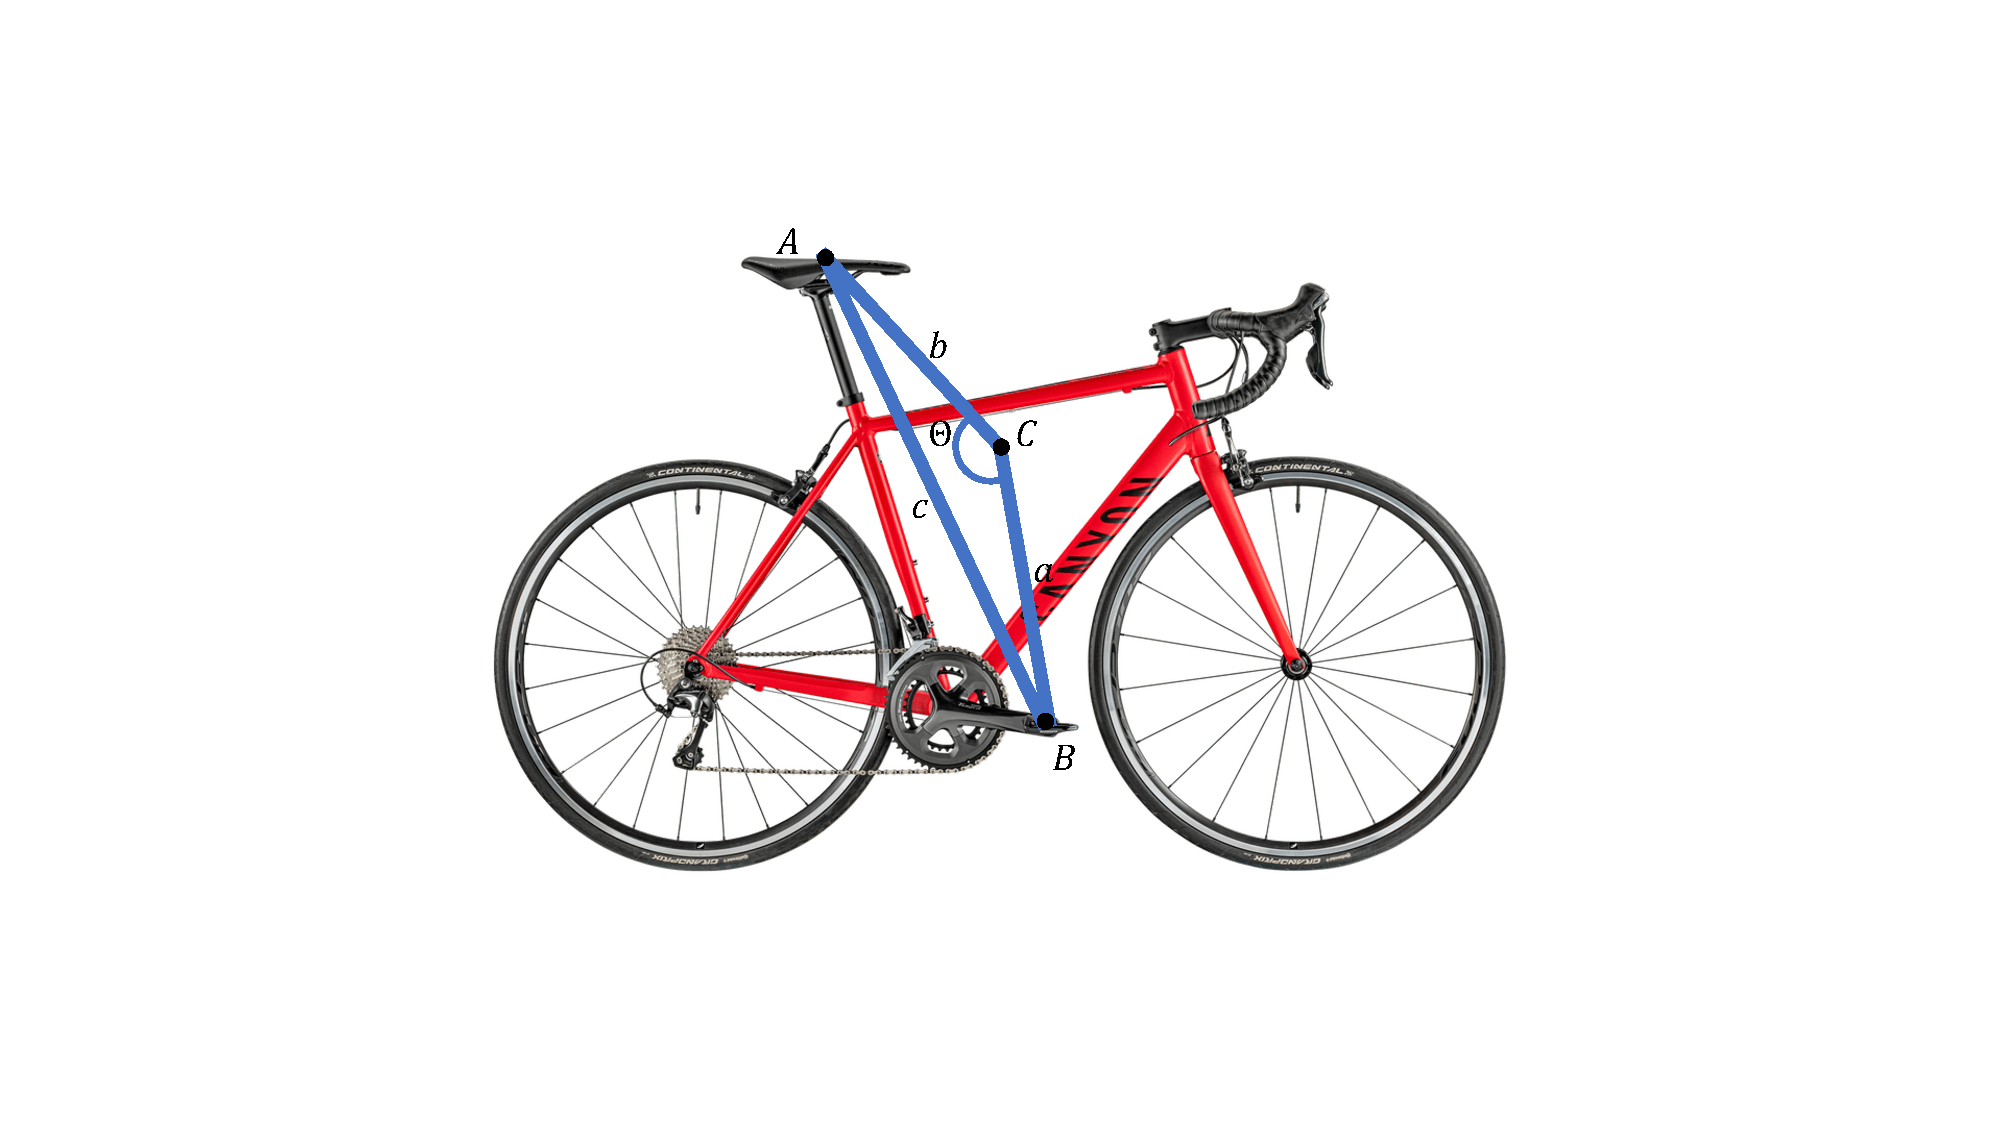
\includegraphics[width=8cm]{fiets.pdf}
	\end{center}
	\caption{Verduidelijkende figuur bij het bepalen van de zadelhoogte. Afbeelding van \href{redbull.com}{Redbull}}
	\label{fiets}
\end{figure}

\subsection{Algoritme voor wijzigen van de stuurpenlengte}

Nu kijken we naar de invloed van de lengte van de stuurpen. Dit heeft vooral invloed op de schouderhoek. Het probleem is dat als we de lengte van de stuurpen willen aanpassen, we een nieuwe stuurpen moeten kopen. Er zijn ook bepaalde grenzen aan de lengte van een stuurpen. De minimale lengte is 40 \si{mm}, korter is bijna onmogelijk. Het maximum ligt rond de 140 \si{mm}, groter kan nog maar dat is heel uitzonderlijk. De output van het algoritme is het aantal \si{cm} dat het stuur naar voor of naar achter moet.


\paragraph{Wiskundige redenering en implementatie}


We willen graag de verandering van de x-coördinaat van de pols (\(B_x\)) berekenen om de gewenste hoek $\theta$ tussen de rug en de arm te bekomen. Hiervoor gebruiken we weer de cosinusregel om de lengte tussen de heup en de pols te bepalen als deze in de goede positie staat.
\[c^2 = a^2 + b^2 -2\cdot a\cdot b\cdot \cos(\theta)\]

Met \(a\) de lengte van de rug, \(b\) de lengte van de arm (schouder tot pols) en \(c\) de lengte tussen de heup en de pols (zie Figuur \ref{stuurpenlengte}). We weten ook dat
\[c^2 = (B_x - A_x)^2 + (B_y - A_y)^2\]

Waaruit volgt dat
\[B_x = \pm \sqrt{c^2 -(B_y - A_y)^2 } + A_x\]

We weten nu welke x-coördinaat de pols moeten hebben om de hoek $\theta$ te bekomen tussen de rug en de arm. Hiermee kunnen we een wijziging in de positie van het stuur voorstellen. Of je een + of - moet nemen hangt af van de richting waarin de persoon op de fiets kijkt.
\begin{figure}[H]
	\begin{center}
		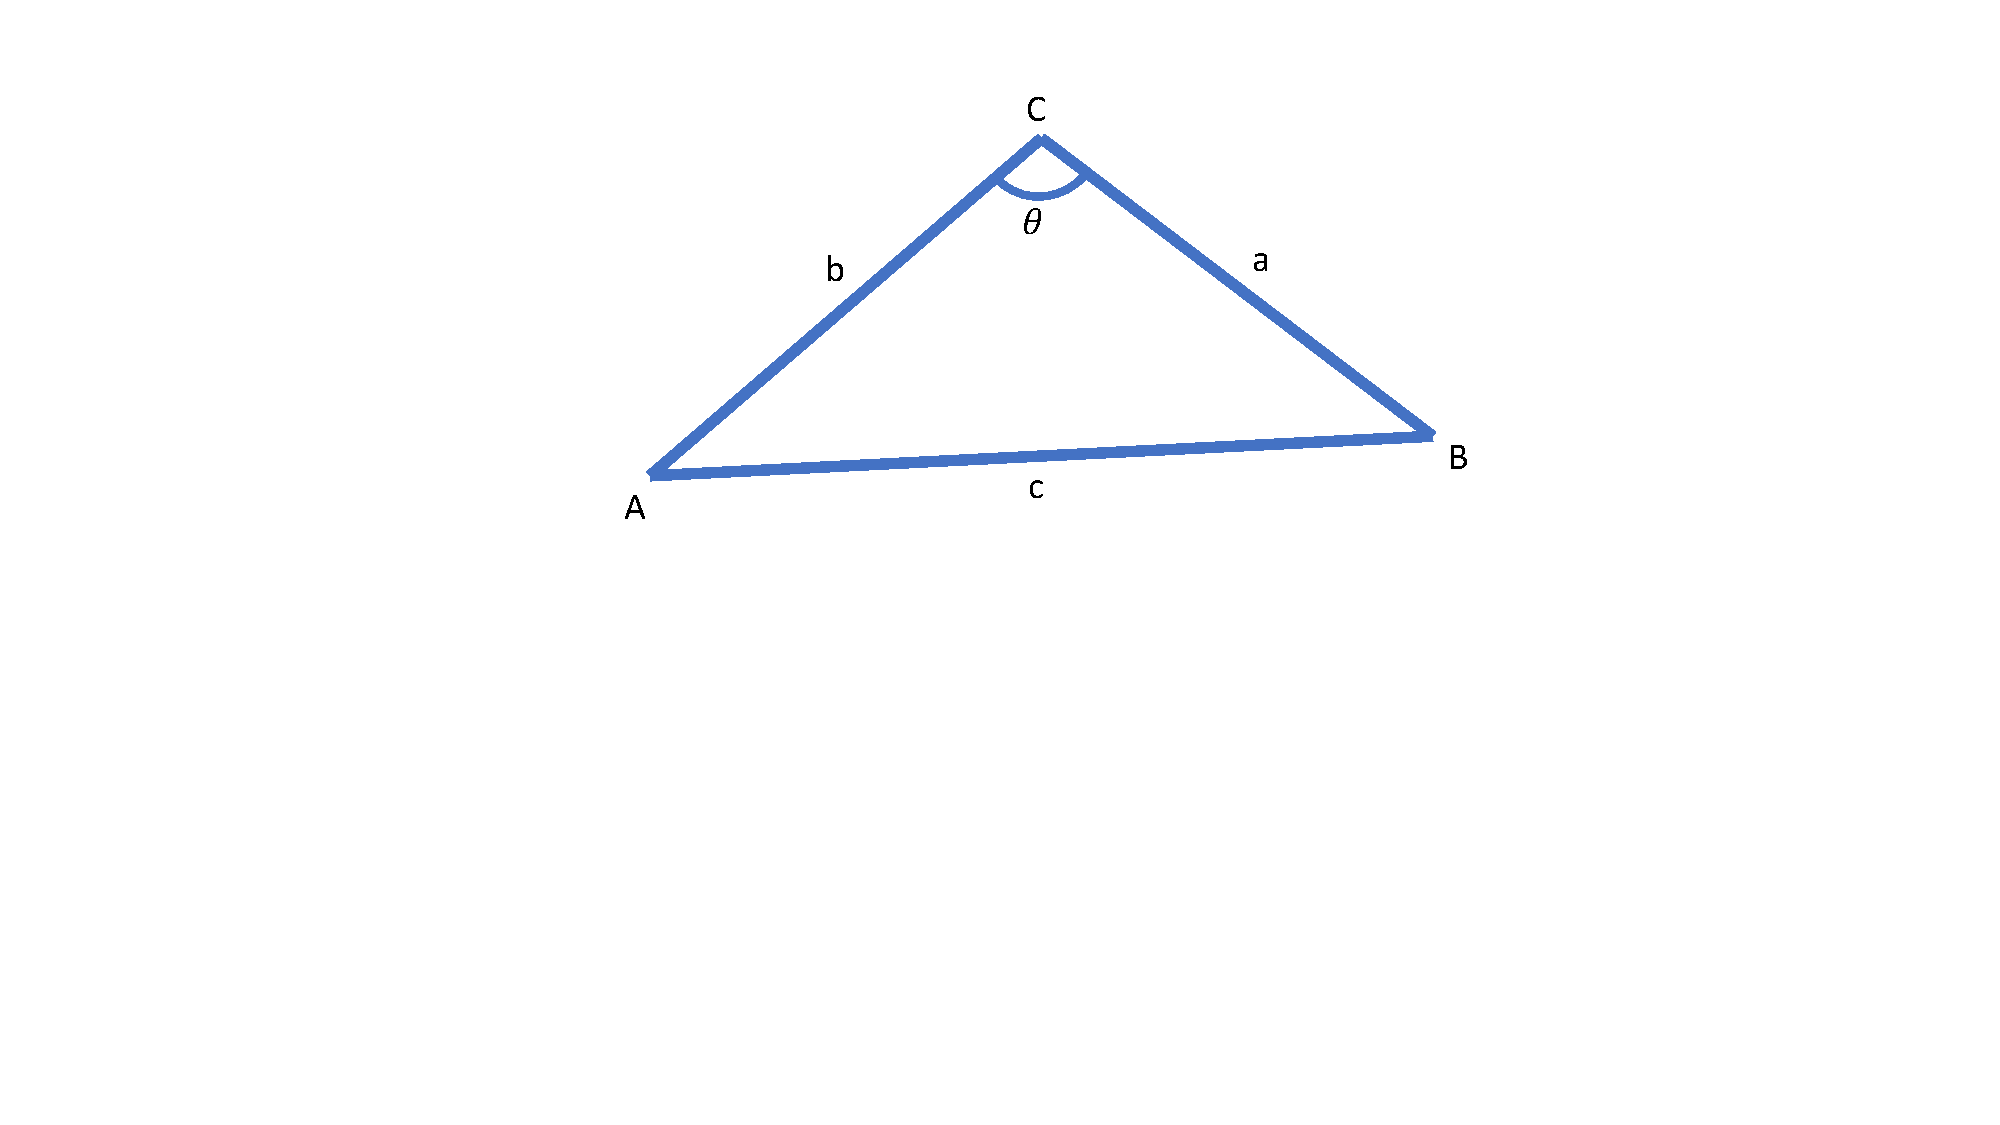
\includegraphics[width=8cm]{yeye.pdf}
	\end{center}
	\caption{Verduidelijkende figuur bij het bepalen van de stuurpenlengte. Afbeelding van \href{redbull.com}{Redbull}}
	\label{stuurpenlengte}
\end{figure}

\subsection{Opmerkingen}

\paragraph{Invloed van de resolutie}
Om de invloed van de resolutie van de genomen foto na te gaan, zijn we gestart met een foto van 1500 op 1500 pixels als referentie. We hebben deze foto herschaald naar foto's van lagere en hogere resoluties. Bij foto's die een hogere resolutie hadden dan 500x500 bleven de hoeken tamelijk stabiel met een maximale spreiding van 2\degree. Bij foto's met een nog kleinere resolutie werd dit al snel 7\degree. Dit is een veel te grote fout voor een \textit{bikefitting}. Als we dan keken naar de afwijking van de voorgestelde verhoging/verlaging van het zadel kwamen we op een veel grotere spreiding. Bij foto's van een resolutie hoger dan 1000x1000 bedroeg de afwijking 2 tot 3 \si{mm}, maar bij lagere resoluties liep dit op tot 5 à 6 \si{mm}. Dit is een veel te grote foutenmarge voor een \textit{bikefitting} waar juist die enkele millimeters bepalend kunnen zijn.

\paragraph{OpenPose maakt slechts een schatting van de positie}
OpenPose kiest niet altijd de \textit{keypoints} juist op de gewrichten omdat het slechts een schatting maakt van de pose. Dit resulteert vaak in een andere waarde voor een hoek dan de werkelijke waarde. Dit vormt een probleem aangezien we de optimale zadelhoogte baseren op werkelijke hoeken. We hebben online een foto van een professionele \textit{bikefitting} gevonden en ons programma daarop laten lopen. Op Figuur \ref{proffessionele_bikefit} is duidelijk te zien dat een afwijking van de \textit{keypoints} een grote invloed heeft op de aanpassingen die ons algoritme voorstelt. Zo ligt het juiste knooppunt van de heup verder naar achter, waardoor de hoek van de knie in het echt scherper is. Het knooppunt van de schouder ligt ook meer naar boven en dat van de arm meer schuin naar boven. Al deze afwijkingen van de \textit{keypoints} geschat door OpenPose zorgen voor fouten op ons algoritme en de aanpassingen die voorgesteld worden.

\begin{figure}[H]
	\centering
	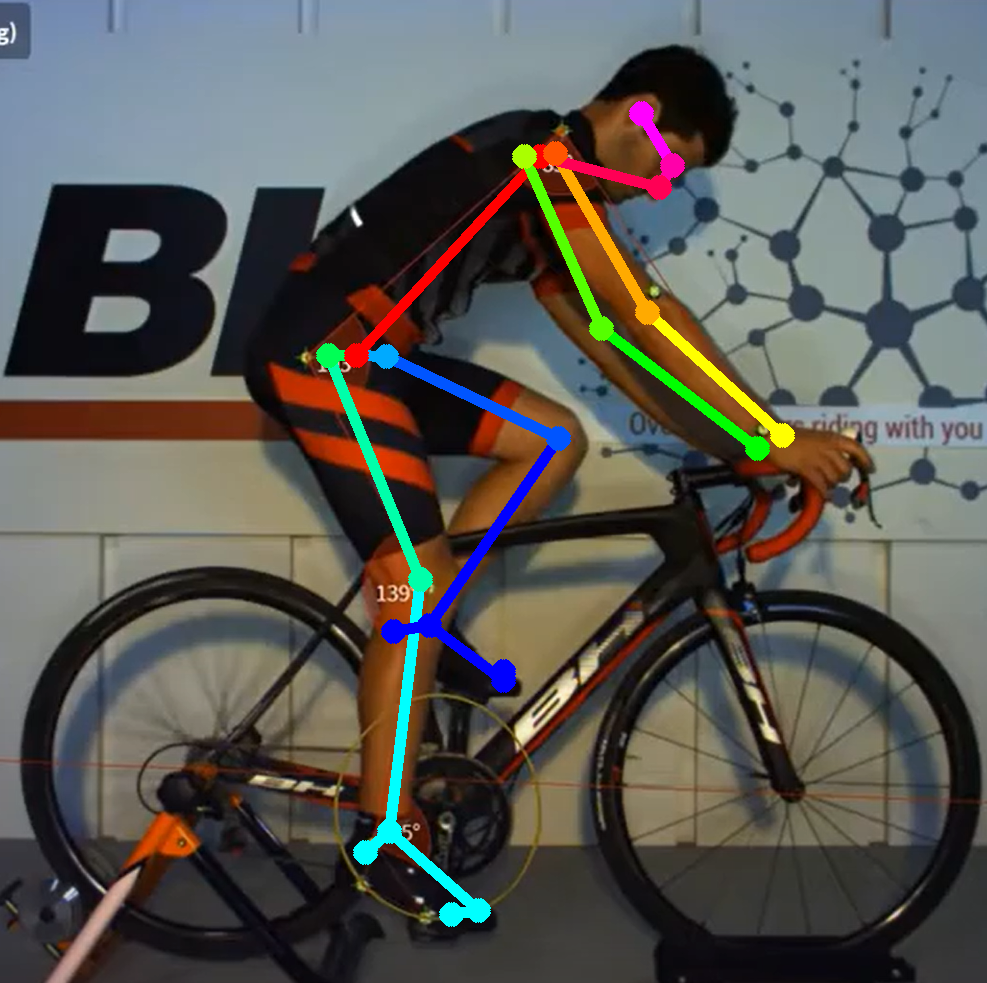
\includegraphics[width= \textwidth]{prof_bikefit}
	
	\caption{foto van professionele \textit{bikefitting} waarop we OpenPose laten lopen hebben om het verschil te analyseren. (screenshot van \href{https://www.youtube.com/watch?v=CTYmJi6zH6oabchannel=STTSystems}{STTSystems op Youtube})}
	\label{proffessionele_bikefit}
\end{figure}

\paragraph{Omzetten van pixels naar centimeter}
De output van OpenPose zijn de coördinaten van de \textit{keypoints}. De eenheid van deze coördinaten zijn echter pixels en is dus relatief ten opzichte van de resolutie van de foto. Om over te gaan naar een absolute eenheid vragen we als input de lengte van het dijbeen die we dan ook kunnen berekenen in OpenPose en zo bepalen we hoeveel pixels er in een \si{cm} gaan. Het grote probleem is nu dat je nooit op dezelfde manier de lengte van je dijbeen zal meten zoals OpenPose die berekent. Als je dus van bij de start al fout gemeten hebt, zal je verder rekenen met fouten en nooit de juiste waarde uitkomen.

\paragraph{Probleem bij bepalen van de schouderhoek}
De ideale schouderhoek is 90\degree. OpenPose ziet de rug echter als een recht stuk terwijl er in het echt wel enige buiging in zit (zie ook Figuur \ref{proffessionele_bikefit}). Daardoor kan de hoek in het echt rond de 90\degree liggen terwijl OpenPose een compleet andere waarde zal geven.

\subsection{Conclusie}
\textit{Bikefitting} is een heel precieze wetenschap. Het gaat om die laatste millimeters waarmee de parameters aangepast worden. We hebben echter gemerkt dat OpenPose hier niet de goeie toepassing voor is om de redenen die hierboven opgelijst staan. We concluderen dus dat een \textit{bikefitting} programma gebaseerd op OpenPose veel te omslachtig is en dat je waarschijnlijk een beter en sneller resultaat zal hebben indien je de zadelhoogte op het gevoel aanpast in de wetenschap dat je knie nog lichtjes gebogen moet zijn als je voet beneden staat.


\section{Toepassing 3: Correct uitvoeren van fitnessoefeningen}

Als derde toepassing maken we een programma dat helpt om op de correcte manier een squat uit te voeren. Dit is meer geschikt voor OpenPose omdat het niet aankomt op millimeters. Als input wordt een collectie foto's van een aantal squats gevraagd. Er wordt dan per squat een score gegeven op basis van een aantal richtlijnen voor het uitvoeren van een goeie squat.\cite{squats} 

\subsection{Richtlijnen voor een goeie squat}

Met OpenPose kunnen we twee parameters goed bepalen.
Ten eerste controleren we de positie van de knie. Deze moet zich op het laagste punt van de squat recht boven de tenen bevinden zoals op Figuur \ref{squat_knie}. Daarnaast moeten ook de heup en de knie zich op dezelfde hoogte bevinden op het laagste punt van de squat zoals op Figuur \ref{squat_heup}. Bij deze twee voorschriften komt het niet aan op millimeters en dus is dit ideaal voor OpenPose. Andere richtlijnen zoals een rechte rug kunnen we moeilijk of niet testen met OpenPose aangezien de rug daar altijd een rechte is.

\begin{figure}[H]
	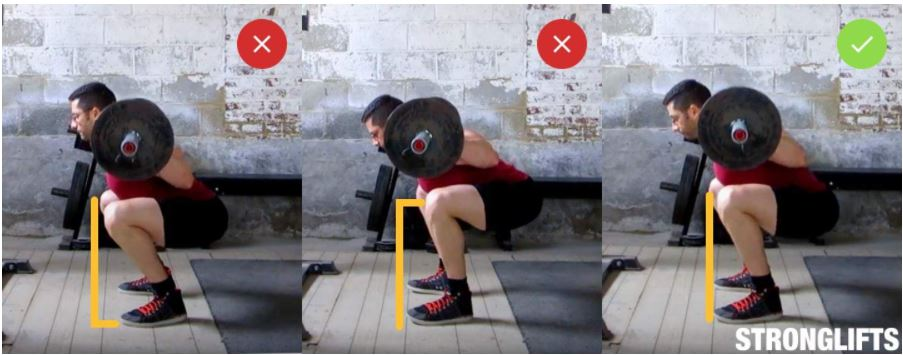
\includegraphics[width= \textwidth]{squat_knie}
	\caption{Op het laagste punt van de squat moet de knie zich recht boven de tenen bevinden. (afbeelding van \cite{squats})}
	\label{squat_knie}
\end{figure}

\begin{figure}[H]
	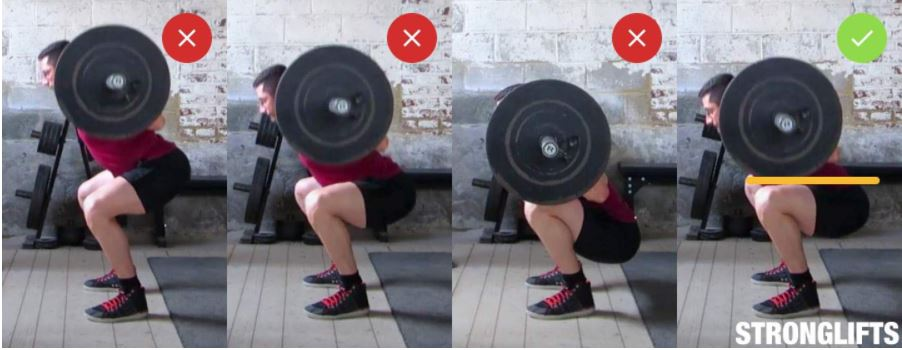
\includegraphics[width= \textwidth]{squat_heup}
	\caption{Op het laagste punt van de squat moeten de heup en knie zich op dezelfde hoogte bevinden. (afbeelding van \cite{squats})}
	\label{squat_heup}
\end{figure}

\subsection{Algoritme voor het bepalen van een goeie squat}
Voor de implementatie van het analyseren van een squat houden we rekening met de twee richtlijnen die we hierboven vermeld hebben. We hebben dus de coördinaten van de knooppunten van de tenen, knie en heup nodig. Voor de eerste richtlijn controleren we dan of de x-coördinaat van de tenen en die van de knie niet te veel verschillen. Voor het tweede voorschrift controleren we of de y-coördinaat van de knie en de heup niet te ver uit elkaar liggen. Op basis van de twee verschillen wordt dan een score voor de squat gegeven.


\subsection{Invloed van camerapositie op output van OpenPose} \label{camerapositie}
In de vorige toepassingen namen we aan dat de foto vanuit een goede positie werd genomen, voor deze toepassing wilden we een concreet antwoord vinden op de vraag: "Wat is het effect van de camerapositie?" Bij het nemen van een foto of video die je wil analyseren zijn er heel wat variabelen: hoe ver je staat, hoe hoog de camera staat en vanuit welke hoek t.o.v. de persoon de foto genomen is. Daarom is het belangrijk dat we testen wat de invloed is van deze variabelen op de uitkomst van ons programma. We hebben dit op een systematische manier getest, zo hoopten we duidelijke conclusies te kunnen trekken uit de data.

\paragraph{Methode}
Eerst werden vijf foto’s genomen vanop één meter afstand recht op de zijkant van de persoon die de squat uitvoert. Deze 5 foto’s zijn op hoogtes van 120, 100, 80, 60 en 40 centimeter genomen. Dit zal zo zijn voor elke reeks. De tweede reeks werd vanop 1,50m afstand genomen en de derde reeks vanop 2m afstand . De vierde en vijfde reeks werden dan weer van 1,50m afstand genomen maar één keer 50cm naar links en de andere keer 50cm naar rechts. Op figuur \ref{cameraopstelling} worden de cameraposities visueel verduidelijkt. Tussen de foto’s van een reeks werd de squatpositie aangehouden en dus amper bewogen, maar tussen de verschillende reeksen kan wel een verschil zitten omdat de squat dan opnieuw werd uitgevoerd. De resultaten zijn te zien in tabel \ref{tabelhoek} en tabel \ref{tabelafstand}. 
\begin{figure}
	\centering
	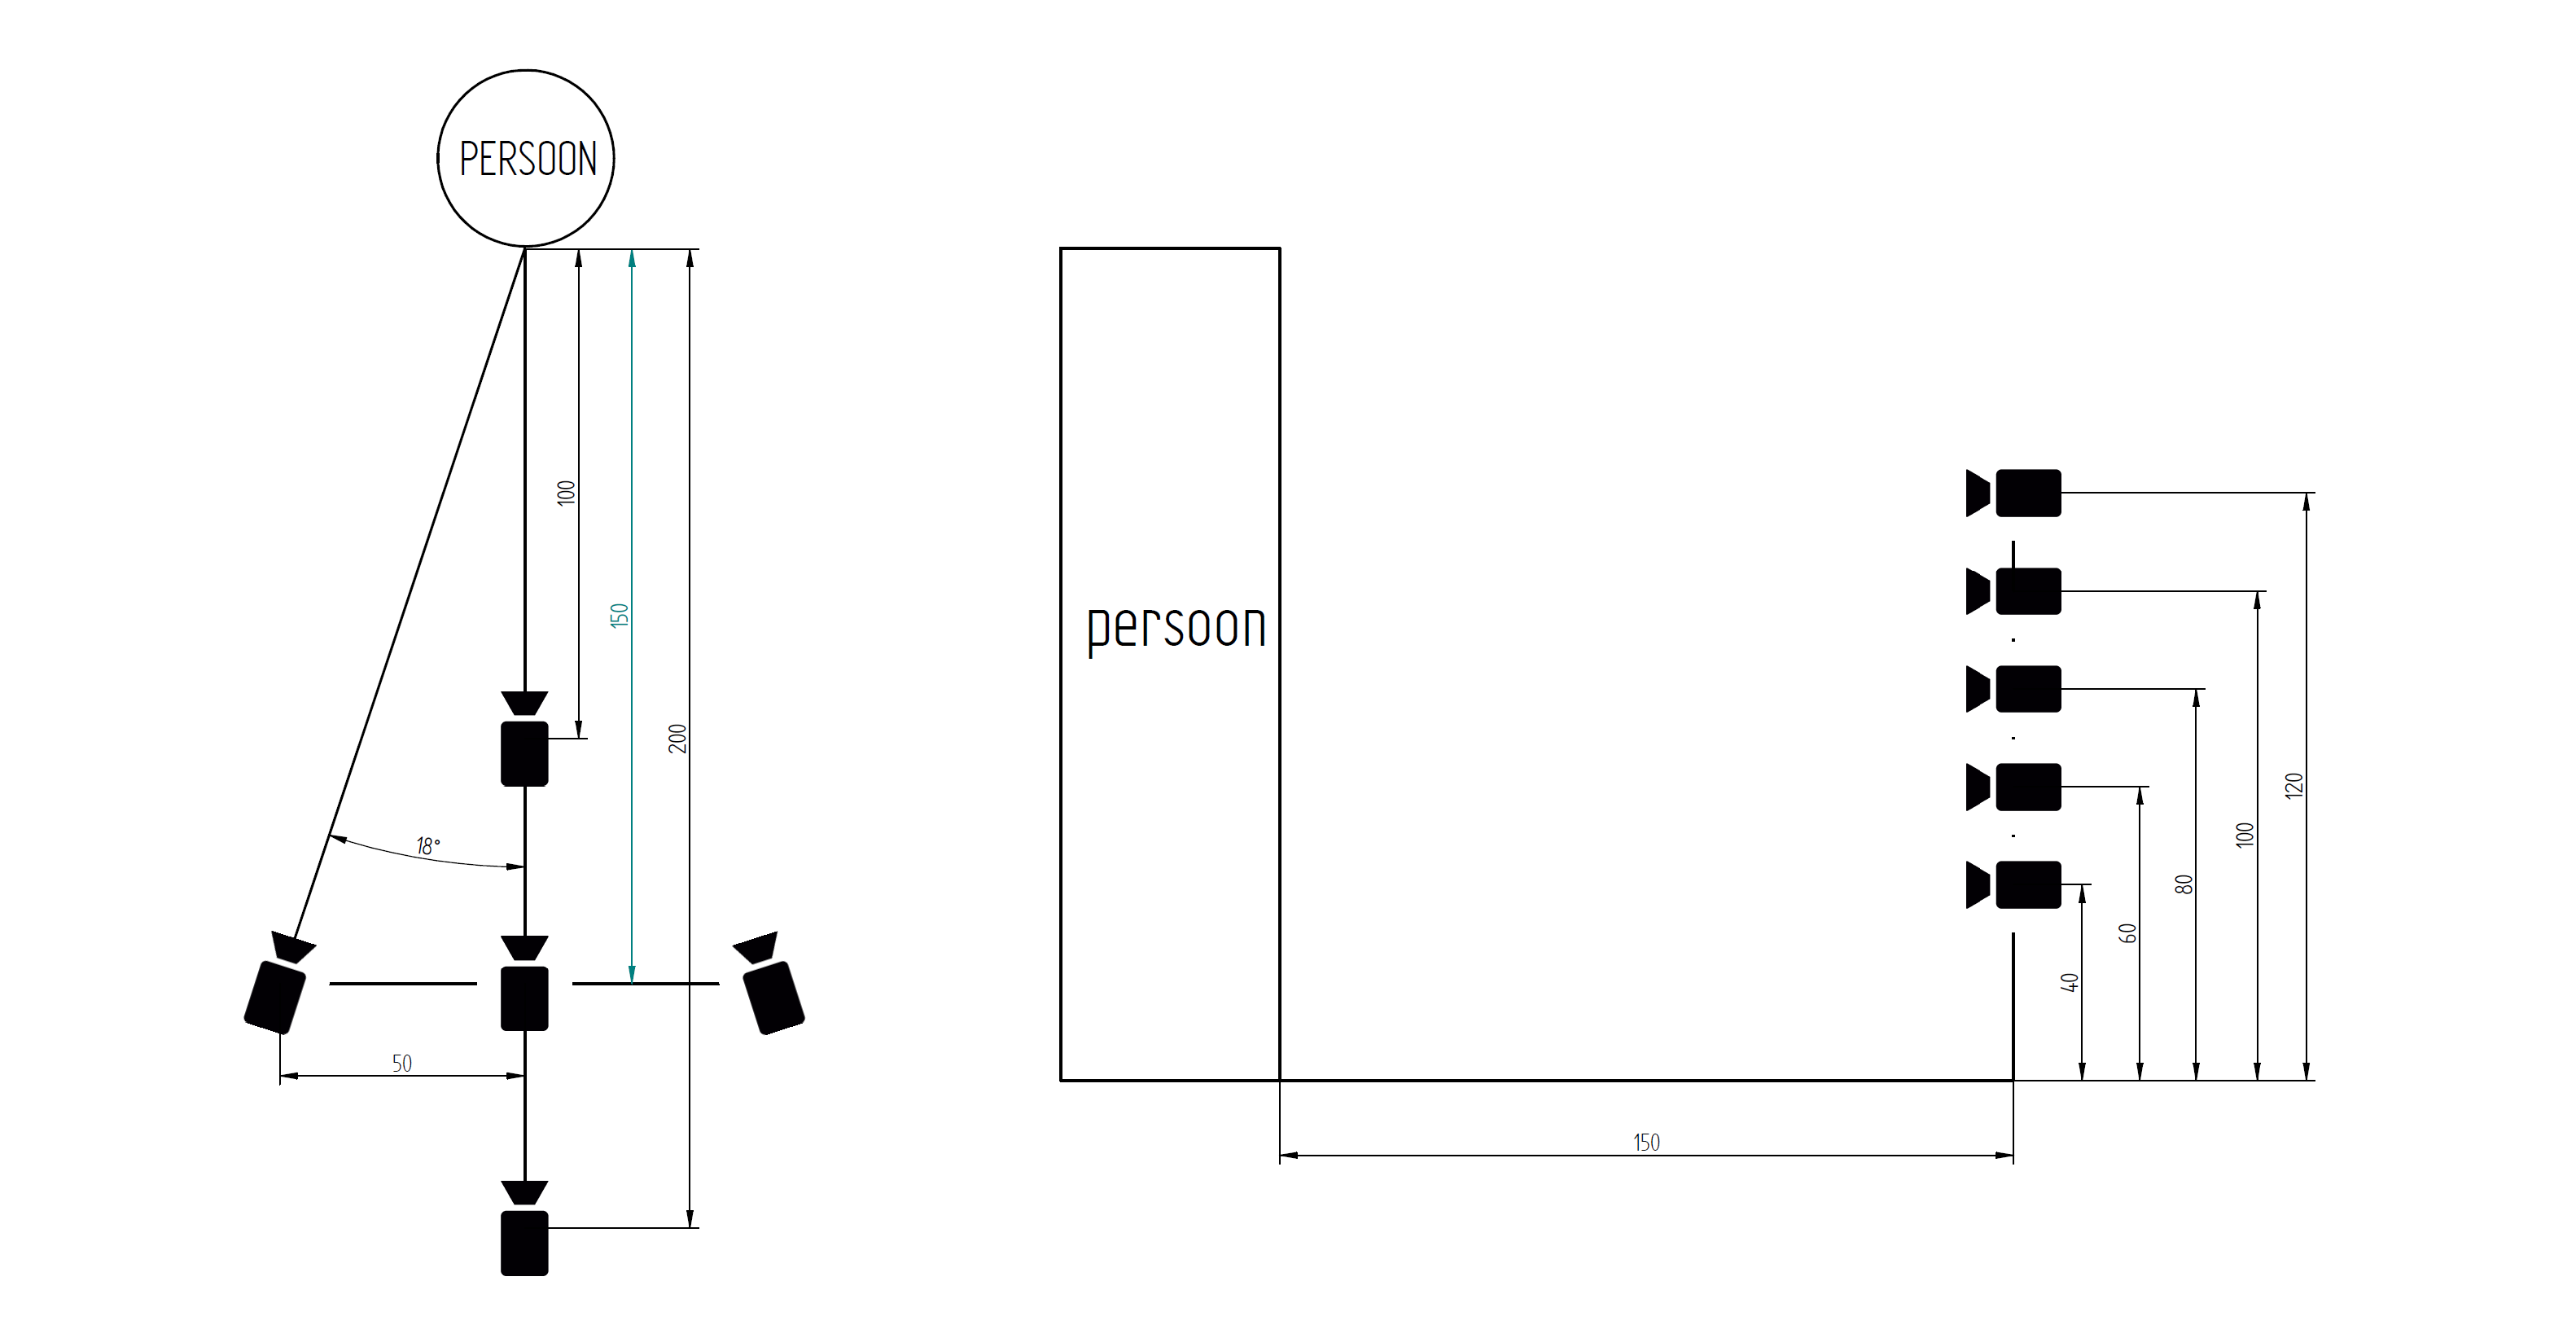
\includegraphics[width=1.2\textwidth]{cameraopstelling}
	\caption{Cameraopstelling gebruikt voor de test. Links is het bovenaanzicht van de 5 verschillende posities vanwaar foto's genomen zijn. De rechter figuur toont het zijaanzicht van de positie recht naast de persoon op 1.50m afstand.}
	\label{cameraopstelling}
\end{figure}

\begin{table}[htbp]
	\centering
	\caption{Hoek van knie gemeten tijdens laagste punt van een squat. De waarden in de tabel zijn de hoeken gemeten van een bepaalde camerapositie (verticaal) en een bepaalde camerahoogte (horizontaal). Alle hoeken zijn uitgedrukt in graden.}
	\begin{tabular}{l|rrrrr} \toprule
		plaats/hoogte & 0,40m & 0,60m & 0,80m & 1,00m & 1,20m\\ \midrule
		1,00m & 83,65 & 84,38 & 84,15 & 79,51 & 80,32 \\
		1,50m & 95,64 & 93,79 & 92,49 & 91,51 & 93,57 \\
		2,00m & 82,11 & 84,33 & 85,40 & 85,36 & 91,22 \\
		links & 91,61 & 92,77 & 93,88 & 95,42 & 93,00 \\
		rechts & 79,34 & 79,49 & 78,26 & 73,88 & 73,92 \\
	\end{tabular}%
	\label{tabelhoek}%
\end{table}%
% Table generated by Excel2LaTeX from sheet 'Blad1'
\begin{table}[htbp]
	\centering
	\caption{Afstand van knie over de voet tijdens het laagste punt van de squat. De waarden in de tabel zijn de afstanden gemeten van een bepaalde camerapositie (verticaal) en een bepaalde camerahoogte (horizontaal). Alle afstanden zijn uitgedrukt in pixels. Het minteken duidt erop dat de knie van de persoon zich voor de voet bevond, zoals de eerste foto op figuur \ref{squat_knie}}
	\begin{tabular}{l|rrrrr}
		plaats/hoogte & \multicolumn{1}{l}{0,40m} & \multicolumn{1}{l}{0,60m} & \multicolumn{1}{l}{0,80m} & \multicolumn{1}{l}{1,00m} & \multicolumn{1}{l}{1,20m} \\\midrule
		1,00m & -113,22 & -96,49 & -50,97 & -90,70 & -62,27 \\
		1,50m & -17,17 & -28,23 & -34,07 & -34,12 & -33,96 \\
		2,00m & -39,58 & -39,90 & -34,00 & -39,64 & -28,36 \\
		links & -11,54 & -11,42 & -16,89 & -28,51 & -17,17 \\
		rechts & -76,85 & -67,82 & -62,46 & -76,54 & -45,47 \\
	\end{tabular}%
	\label{tabelafstand}%
\end{table}%

\paragraph{Besluit}
De afstanden werden steeds afgemeten maar kunnen meetfouten bevatten. Ook de kanteling van de camera was niet consistent wat heel wat invloed had op de data. Hierdoor is het moeilijk om een duidelijk besluit te kunnen nemen. Omdat OpenPose in 2D werkt en je hoeken en afstanden meet van een 3D object, hebben we te maken met een projectie, wat heel wat distorsie met zich meebrengt. Bij deze testen hebben we dit ook gemerkt, zelfs als we proberen de foto’s op een systematische manier te nemen zodat we mogelijks verbanden kunnen zien. Ook het feit dat de positie niet perfect gelijk is tussen de reeksen foto’s maakt het moeilijk om conclusies te trekken. Als je de data bekijkt, is het duidelijk dat de hoeken en afstanden heel willekeurig veranderen. Hierdoor is het niet mogelijk het exacte effect van de cameraposities te achterhalen. Wel is het logisch dat een foto recht voor de persoon een realistischer beeld en resultaat zal geven dan een foto die vanuit een grote hoek is genomen. Hoe ver je staat van de persoon maakt ook niet zoveel uit, het is gewoon belangrijk dat de volledige persoon in beeld is, want anders heeft OpenPose minder data om mee te werken.

\chapter*{Besluit}

Over het algemeen kunnen we besluiten dat OpenPose een heel handige \textit{tool} is voor positiebepaling. Het is inzetbeer in tal van toepassingen, maar uit dit verslag blijkt dat het toch geen wonderoplossing is die alle problemen oplost. Uit onze eerste toepassing, waarbij we de schouderhoek meten, hebben we geleerd dat het heel makkelijk is om te werken met de output van OpenPose. Onze tweede toepassing, de \textit{bikefit}, hebben we verder uitgewerkt en zo ontdekten we heel wat struikelblokken. Het is duidelijk dat de output van OpenPose wordt beïnvloed door heel wat variabelen zoals de camerapositie en resolutie. Ook bij het omzetten van de data naar bruikbare eenheden worden steeds nieuwe fouten geïntroduceerd. Door al deze dingen samen moeten we concluderen dat OpenPose geen oplossing biedt op vlak van \textit{bikefitting}. Aangezien het hier om precieze metingen gaat kunnen we deze conclusie verder trekken en concluderen dat OpenPose niet goed is voor toepassingen die steunen op nauwkeurigheid. Als laatste probeerden we met OpenPose een squat te beoordelen en dit was heel succesvol. We hebben hier dan ook de invloed van de camerapositie concreet getest. De conclusie is dat je best de foto's neemt loodrecht op het vlak van de hoek of hoeken die je wil meten. \\
Tijdens dit project zijn we op zoek gegaan naar de limieten van OpenPose en momenteel is het dus niet bruikbaar voor nauwkeurige toepassingen. Maar de vooruitgang op vlak van artificiële intelligentie en neurale netwerken verzekert een goede toekomst voor OpenPose. Daarom geloven wij dat het later nog breder toepasbaar zal worden.



\bibliographystyle{unsrt}
\bibliography{bibliografie}
%\printindex

\chapter*{Vakintegratie}
Het is belangrijk om dit project een plaats te geven binnen onze opleiding ingenieurswetenschappen. We bekijken welke vakken uit de eerste 3 semesters van onze bachelor het meest gebruikt worden tijdens dit project. De belangrijkste link is met het vak beginselen van programmeren. In dit vak leerden we werken met Python en verworven we inzicht in het programmeren. Wat heel handig is, want tijdens ons project maken we veelvuldig gebruik van Python. Elk zelfgemaakt programma is geschreven in Python want OpenPose heeft een uitstekende Python API. Verder maakt wiskunde ook een groot deel uit van ons project, want het berekenen van hoeken of afstanden kan niet zonder de wiskunde. We gebruiken hierbij kennis uit verschillende wiskundige vakken zoals, Analyse \& calculus en Lineaire algebra. Als laatste kunnen we Statistiek ook nog linken aan dit project aangezien OpenPose enkel een schatting geeft van de lichaamspositie. Het werkt met \textit{heatmaps} en kiest per knooppunt dan het coördinaat met de hoogste kans. We gebruiken zelf geen statistische technieken, maar het helpt ons wel bij het begrijpen van OpenPose.

\chapter*{Planning}

\begin{landscape}
	\begin{figure}
		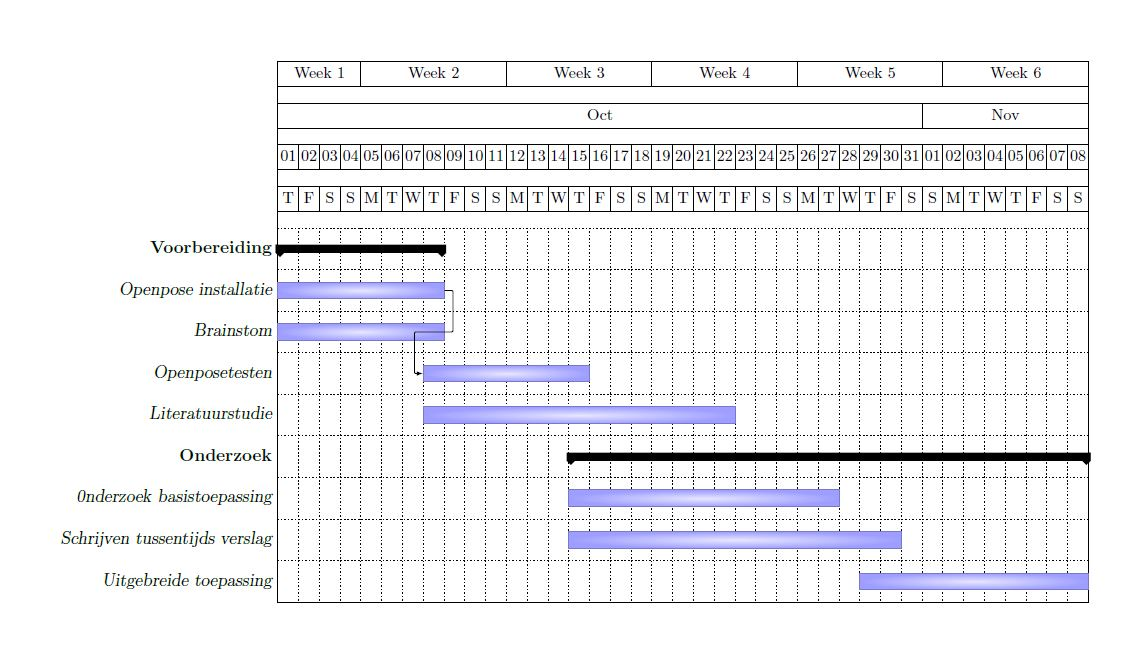
\includegraphics[width= 2\textwidth]{ganttchart_1}
	\end{figure}
	\begin{figure}
		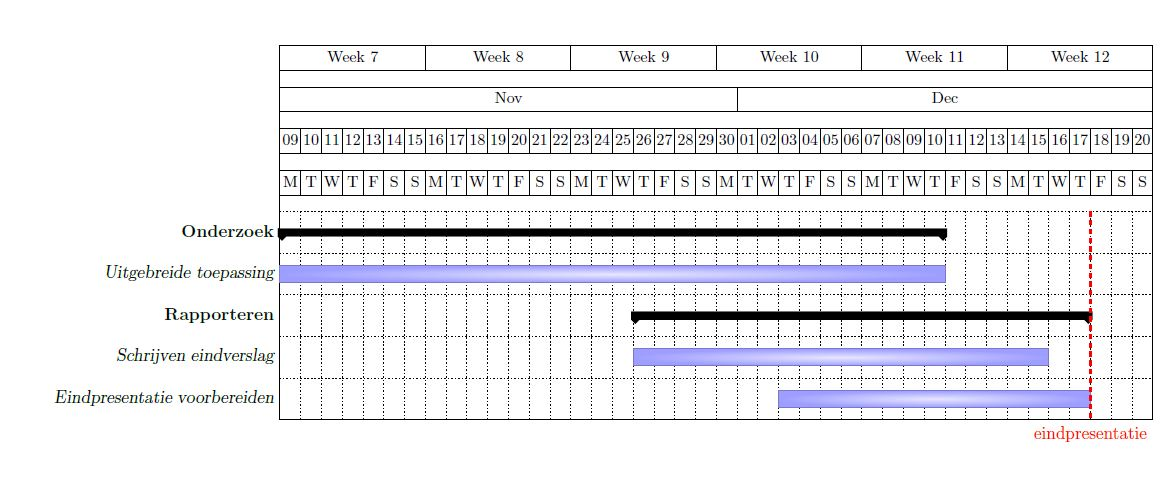
\includegraphics[width= 2\textwidth]{ganttchart_2}
	\end{figure}
\end{landscape}

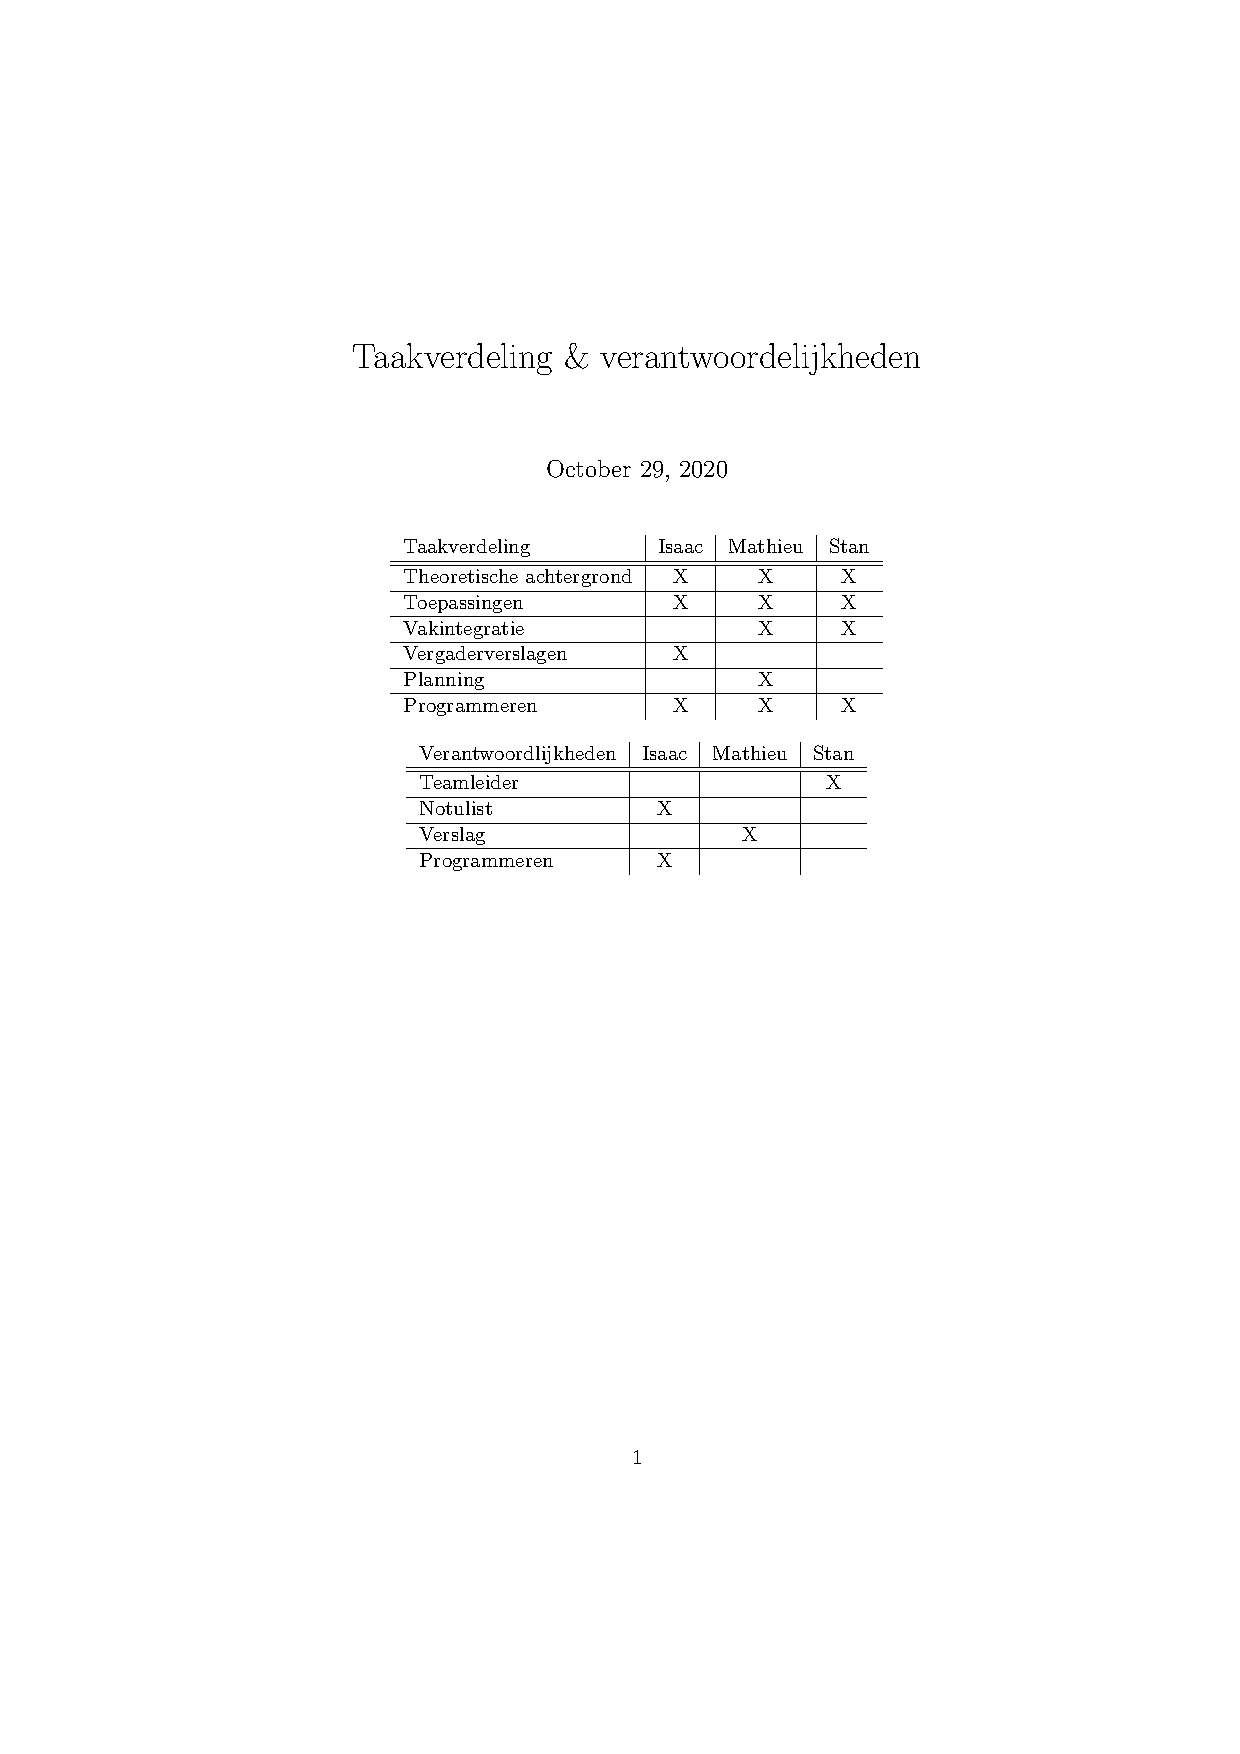
\includepdf{taakverdeling.pdf}

\end{document}